\documentclass[11pt,a4paper,oneside,openany]{memoir}

\usepackage{preamble}
% Notation used throughout. Defined once; every chapter draws from here.

% === sets and spaces ===
\newcommand{\R}{\mathbb{R}}
\newcommand{\N}{\mathbb{N}}
\newcommand{\Z}{\mathbb{Z}}
\newcommand{\C}{\mathbb{C}}
\newcommand{\Rd}[1][d]{\mathbb{R}^{#1}}
\newcommand{\Sph}{\mathbb{S}}
\newcommand{\dom}{\mathcal{X}}
\newcommand{\lab}{\mathcal{Y}}
\newcommand{\Hil}{\mathcal{H}}

% === probability ===
\DeclareMathOperator*{\Ex}{\mathbb{E}}
\DeclareMathOperator*{\Var}{Var}
\DeclareMathOperator*{\Cov}{Cov}
\DeclareMathOperator*{\argmin}{arg\,min}
\DeclareMathOperator*{\argmax}{arg\,max}
\newcommand{\given}{\,|\,}
\newcommand{\dist}{\sim}
\newcommand{\KL}[2]{D_{\mathrm{KL}}\!\left(#1 \,\|\, #2\right)}
\newcommand{\Normal}{\mathcal{N}}
\newcommand{\Unif}{\mathrm{Unif}}
\newcommand{\pdata}{p_{\mathrm{data}}}
\newcommand{\MSE}{\mathrm{MSE}}
\newcommand{\bias}{\mathrm{bias}}

% === linear algebra and calculus ===
\newcommand{\T}{^{\mathsf{T}}}
\newcommand{\inv}{^{-1}}
\newcommand{\grad}{\nabla}
\newcommand{\Hess}{\mathbf{H}}
\newcommand{\norm}[1]{\left\lVert #1 \right\rVert}
\newcommand{\abs}[1]{\left\lvert #1 \right\rvert}
\newcommand{\inner}[2]{\left\langle #1, #2 \right\rangle}
\newcommand{\vect}[1]{\mathbf{#1}}
\newcommand{\mat}[1]{\mathbf{#1}}
\newcommand{\id}{\mathbf{I}}
\newcommand{\tr}{\operatorname{tr}}
\newcommand{\diag}{\operatorname{diag}}
\newcommand{\spn}{\operatorname{span}}
\newcommand{\rank}{\operatorname{rank}}

% === learning ===
\newcommand{\params}{\theta}
\newcommand{\wt}{\vect{w}}
\newcommand{\xin}{\vect{x}}
\newcommand{\yout}{\vect{y}}
\newcommand{\Loss}{\mathcal{L}}
\newcommand{\risk}{\mathcal{R}}
\newcommand{\net}{f_{\params}}
\newcommand{\lr}{\eta}
\newcommand{\est}[1]{\widehat{#1}}
\newcommand{\sigmoid}{\sigma}

% === representations, alignment (Isola) ===
\newcommand{\rep}{\phi}
\newcommand{\repB}{\psi}
\newcommand{\kernel}{K}
\newcommand{\CKA}{\mathrm{CKA}}
\newcommand{\Hcent}{\mathbf{H}}   % centring matrix
\newcommand{\simfn}{s}

% === diffusion (Dieleman) ===
\newcommand{\xz}{\vect{x}_0}
\newcommand{\xt}{\vect{x}_t}
\newcommand{\eps}{\boldsymbol{\varepsilon}}
\newcommand{\epsnet}{\eps_{\params}}
\newcommand{\snr}{\mathrm{SNR}}
\newcommand{\score}{\grad_{\xt} \log p_t(\xt)}
\newcommand{\guide}{w}

% === reinforcement learning (Deac) ===
\newcommand{\st}{s_t}
\newcommand{\at}{a_t}
\newcommand{\rt}{r_t}
\newcommand{\States}{\mathcal{S}}
\newcommand{\Actions}{\mathcal{A}}
\newcommand{\Trans}{P}
\newcommand{\Rew}{R}
\newcommand{\disc}{\gamma}
\newcommand{\pol}{\pi_{\params}}
\newcommand{\traj}{\tau}
\newcommand{\ret}{G}
\newcommand{\Vf}{V}
\newcommand{\Qf}{Q}
\newcommand{\Adv}{A}
\newcommand{\obj}{J}

% === geometric deep learning (Velickovic) ===
\newcommand{\Grp}{\mathfrak{G}}
\newcommand{\grp}{\mathfrak{g}}
\newcommand{\Om}{\Omega}
\newcommand{\Sig}{\mathcal{X}}
\newcommand{\gact}[2]{#1 \cdot #2}
\newcommand{\nbr}[1]{\mathcal{N}_{#1}}
\newcommand{\msg}{\psi}
\newcommand{\upd}{\phi}
\newcommand{\agg}{\bigoplus}

% === graph signal processing (Stankovic) ===
\newcommand{\Adj}{\mathbf{A}}
\newcommand{\Lap}{\mathbf{L}}
\newcommand{\GFT}{\mathrm{GFT}}
\newcommand{\eig}{\lambda}
\newcommand{\Vmat}{\mathbf{V}}
\newcommand{\Lam}{\boldsymbol{\Lambda}}
\newcommand{\gsig}{\vect{x}}
\newcommand{\azp}{\Adj_{\mathrm{ZP}}}

% === quantization (Alistarh) ===
\newcommand{\quant}{Q}
\newcommand{\dw}{\delta\wt}
\newcommand{\PPL}{\mathrm{PPL}}

% === continual learning (Lyle, Pascanu) ===
\newcommand{\task}{\mathcal{T}}
\newcommand{\plast}{\kappa}


\addbibresource{refs.bib}

\title{\Huge EEML 2026\\[4pt] \Large Lecture Notes}
\author{Asen Popov}
\date{Cetinje, Montenegro \\ 27 July to 1 August 2026}

\begin{document}

\frontmatter
\maketitle

\begin{KeepFromToc}
\tableofcontents
\end{KeepFromToc}

\mainmatter

\chapter{Overview}
\label{ch:00-overview}

These are summary notes from EEML 2026, the Eastern European Machine Learning Summer School, held in
Cetinje, Montenegro from 27 July to 1 August 2026. They are built from the slide decks distributed
during the week, photographs of the two lectures where no deck was given, four tutorial notebooks,
and two files of personal notes. They are not a transcript. Each lecture chapter states what the
lecture is taken to be arguing, gives the three to six ideas that carry that argument with the
mathematics where the mathematics is the point, and closes by locating the lecture among the
others.

Everything substantive traces back to the materials. Connective reasoning that does not come from a
lecture is confined to marked boxes like the one at the end of this chapter, so it is always visible
which claims belong to a speaker and which do not.

\section*{The week}

\begin{center}
\small
\begin{tabularx}{\textwidth}{@{}l l X l@{}}
\toprule
\textbf{Day} & \textbf{Chapter} & \textbf{Lecture and speaker} & \textbf{Source} \\
\midrule
Mon 27 Jul & \ref{ch:01-intro-deep-learning} & Introduction to Deep Learning, Sarath Chandar
  & photos \\
           & \ref{ch:02-representational-geometry} & Representational Geometry and Alignment,
  Phillip Isola & deck \\
           & \ref{ch:03-diffusion-models} & Diffusion Models, Sander Dieleman & deck \\
Tue 28 Jul & \ref{ch:04-intro-reinforcement-learning} & Introduction to Reinforcement Learning,
  Andreea Deac & slides \\
           & \ref{ch:05-statistics-estimation} & Statistics: Learning to Estimate,
  Kyunghyun Cho & deck \\
Wed 29 Jul & \ref{ch:06-continual-learning} & Continual Learning, Clare Lyle & deck \\
           & \ref{ch:07-to-be-figured-out} & To Be Figured Out, Razvan Pascanu & deck \\
Thu 30 Jul & \ref{ch:08-ml-for-mathematics} & ML for Mathematics, Matija Tapu\v{s}kovi\'{c}
  & deck \\
Fri 31 Jul & \ref{ch:09-spectral-analysis-dags} & Spectral Analysis of DAGs,
  Isidora Stankovi\'{c} & deck \\
           & \ref{ch:10-efficient-learning} & Computationally-Efficient Learning, Dan Alistarh
  & photos \\
Sat 1 Aug  & \ref{ch:11-geometric-deep-learning} & Geometric Deep Learning,
  Petar Veli\v{c}kovi\'{c} & deck \\
\bottomrule
\end{tabularx}
\end{center}

\noindent Four tutorial notebooks accompanied the week, on reinforcement learning, multimodal
learning, mechanistic interpretability and model quantization. They are not written up here,
since the notebooks are self-contained and are better worked through directly. Where a lecture
chapter has a matching tutorial, it says so.

\section*{Where to start}

On a return to this material after some time, the three synthesis chapters at the end are the point
of the exercise and the lecture chapters are their evidence. Chapter~\ref{ch:themes} identifies the
six ideas that recurred, including a genuine disagreement between Lyle and Pascanu about how serious
the i.i.d.\ assumption is. Chapter~\ref{ch:research-directions} separates problems the speakers
flagged as open from directions inferred here. Chapter~\ref{ch:revisit} is an ordered queue of
specific items to return to, with a reason for each.

\begin{aside}
This box is the mechanism for marking editorial additions, so here is one about the notes
themselves. The two lectures with no distributed deck, Chapters~\ref{ch:01-intro-deep-learning}
and~\ref{ch:10-efficient-learning}, are reconstructed entirely from photographs of projected slides,
and although the transcriptions were made at full resolution and are legible, those two chapters
rest on a single source with nothing to corroborate them. The lectures with both a deck and
photographs are the best evidenced, and there the photographs were left untranscribed because the
deck supersedes them.
\end{aside}


\part{Lectures}
\chapter{Introduction to Deep Learning}
\label{ch:01-intro-deep-learning}

\lecturemeta{Sarath Chandar}{Polytechnique Montr\'{e}al and Mila}

The lecture is organised around a single asymmetry: we have known since the early 1990s
what a neural network \emph{can} represent, and we still do not know what we can reliably
\emph{train}. Chandar spends the first half establishing the representational result, the
universal approximation theorem, in order to set it aside, and the second half on the
obstructions that survive it: gradients that vanish through depth, initialisations that
decide whether a network trains at all, and finally the independence assumption buried in
every objective on the slides. The closing frame is the argument of the whole summer school
in one line: current practice optimises the i.i.d.\ case, while ``true learning'' is
sequential, online and continual.

\section*{Key ideas}

\paragraph{The gradient that cancels.} The derivation that opens the lecture is a single
sigmoid unit, $y^{(n)} = \sigmoid(a^{(n)})$ with $a^{(n)} = \wt\T\xin^{(n)}$, trained on
the cross-entropy objective
\[
  \min_{\wt} \; -\sum_{n=1}^{N} \Bigl[ t^{(n)} \ln y^{(n)}
    + \bigl(1 - t^{(n)}\bigr) \ln\bigl(1 - y^{(n)}\bigr) \Bigr],
  \qquad
  \frac{\partial \mathrm{obj}}{\partial \wt}
   = \sum_{n=1}^{N} \frac{\partial \mathrm{obj}}{\partial y^{(n)}}
     \frac{\partial y^{(n)}}{\partial a^{(n)}}
     \frac{\partial a^{(n)}}{\partial \wt}.
\]
\noindent Worked factor by factor, the objective contributes
$\partial \mathrm{obj} / \partial y^{(n)} = (y^{(n)} - t^{(n)}) / (y^{(n)}(1 - y^{(n)}))$,
the unit contributes $\partial y^{(n)} / \partial a^{(n)} = y^{(n)}(1 - y^{(n)})$, and the
pre-activation contributes $\partial a^{(n)} / \partial \wt = \xin^{(n)}$. The awkward
denominator is exactly the sigmoid derivative, so the two cancel, as the board shows by
striking them out, and each term of the sum collapses to
\[
  \bigl(y^{(n)} - t^{(n)}\bigr)\xin^{(n)}.
\]
\noindent Residual times input. The cancellation is the point: it is why this pairing of
output unit and loss is the one everybody uses, and it is the atom that backpropagation
chains.

\paragraph{Backpropagation has a messy provenance.} The slides are unusually careful here, and they
begin further back than most treatments: the perceptron in 1957~\citep{rosenblatt1958}, logistic
regression in 1958~\citep{cox1958}, and the XOR counterexample in 1969~\citep{minsky1969}.
Backpropagation was then popularised by Rumelhart, Hinton and Williams in
1986~\citep{rumelhart1986}, but Werbos had it in 1974~\citep{werbos1974}, and the slide
states flatly that it ``has been reinvented several times before 1986'', pointing at
Schmidhuber's history page~\citep{schmidhuber2014backprop}. What actually changed the field
was not the rule but the tooling, and Chandar gives the timeline: Torch (2002), Theano
(2007 to 2008), Caffe (2013), TensorFlow (2015), PyTorch (2016) and JAX (2018). Automatic
differentiation, not the chain rule, is the enabling technology.

\paragraph{Expressivity is settled.} The universal approximation theorem is quoted as
Hornik, 1991~\citep{hornik1991}: a single hidden layer network with a linear output unit can
approximate any continuous function arbitrarily well, \emph{given enough hidden units}. On
the slide the final clause is highlighted and braced, and underneath, in red, sits the
phrase that reframes everything after it: \textbf{expressivity versus learnability}. One
hidden layer suffices in principle, which is precisely why the rest of the lecture is about
optimisation rather than architecture.

\paragraph{Learnability is not.} Depth turns the chain rule into a product of Jacobians,
\[
  \frac{\partial E}{\partial \mat{W}^{(T)}}
   = \frac{\partial E}{\partial \yout}\,
     \frac{\partial \yout}{\partial \vect{h}_T}
     \underbrace{\left[
       \frac{\partial \vect{h}_T}{\partial \vect{h}_{T-1}}
       \frac{\partial \vect{h}_{T-1}}{\partial \vect{h}_{T-2}} \cdots
       \frac{\partial \vect{h}_2}{\partial \vect{h}_1}
     \right]}_{\text{vanishing gradient problem}},
\]
\noindent and the bracket is boxed on the board. The historical answer was to avoid
training the depth all at once: greedy layerwise pretraining~\citep{hinton2006, bengio2007},
in which each layer is fitted as an autoencoder before the stack is finetuned end to end
(Figure~\ref{fig:intro-deep-learning-1}). The modern answer is quieter and lives in the
activation function, where the lecture records
$\mathrm{Swish}(x) = x\,\sigmoid(x)$~\citep{ramachandran2017} and
$\mathrm{SwiGLU}(x) = \mathrm{Swish}(x\mat{W}) \otimes x\mat{V}$~\citep{shazeer2020}.

\begin{figure}[htbp]
\centering
\begin{tikzpicture}[
  x=1cm, y=1cm, font=\small,
  box/.style={draw, rounded corners=1pt, minimum height=8mm, minimum width=7mm,
              inner sep=1pt, fill=white},
  hid/.style={box, fill=asidebg},
  ar/.style={-{Latex[length=1.6mm]}, shorten >=1pt, shorten <=1pt}]

  \node[box] (x1) at (0,0) {$\xin$};
  \node[hid] (h1) at (1.6,0) {$\vect{h}_1$};
  \node[box] (xr) at (3.2,0) {$\est{\xin}$};
  \draw[ar] (x1) -- node[above,font=\scriptsize] {$\mat{W}^{(1)}$} (h1);
  \draw[ar] (h1) -- node[above,font=\scriptsize] {$\mat{W}^{(1)\mathsf{T}}$} (xr);
  \node[font=\scriptsize, align=center] at (1.6,-1.05)
    {train layer 1 as an autoencoder,\\ reconstructing the input};

  \node[box] (x2) at (6.3,0) {$\xin$};
  \node[hid] (h1b) at (7.9,0) {$\vect{h}_1$};
  \node[hid] (h2) at (9.5,0) {$\vect{h}_2$};
  \node[box] (hr) at (11.1,0) {$\est{\vect{h}}_1$};
  \draw[ar] (x2) -- (h1b);
  \draw[ar] (h1b) -- node[above,font=\scriptsize] {$\mat{W}^{(2)}$} (h2);
  \draw[ar] (h2) -- (hr);
  \node[font=\scriptsize, align=center] at (8.7,-1.05)
    {repeat upward: each new layer\\ reconstructs the one below};

  \node[box] (x3) at (2.2,-3.0) {$\xin$};
  \node[hid] (s1) at (3.8,-3.0) {$\vect{h}_1$};
  \node[hid] (s2) at (5.4,-3.0) {$\vect{h}_2$};
  \node (dots) at (6.7,-3.0) {$\cdots$};
  \node[hid] (sL) at (8.0,-3.0) {$\vect{h}_L$};
  \node[box] (y3) at (9.6,-3.0) {$\yout$};
  \draw[ar] (x3) -- (s1); \draw[ar] (s1) -- (s2); \draw[ar] (s2) -- (dots);
  \draw[ar] (dots) -- (sL); \draw[ar] (sL) -- (y3);
  \draw[decorate, decoration={brace, amplitude=4pt, mirror}]
    (1.75,-3.6) -- (10.05,-3.6)
    node[midway, below, yshift=-3pt, font=\scriptsize] {supervised finetuning};
\end{tikzpicture}
\caption{Greedy layerwise pretraining as drawn in the Introduction to Deep Learning
lecture. Each layer is first trained to reconstruct the representation below it, so no
gradient ever has to travel the full depth, and only then is the assembled stack finetuned
against labels. Redrawn from photographs of the board.}
\label{fig:intro-deep-learning-1}
\end{figure}

\paragraph{Initialisation decides trainability.} The lottery ticket
hypothesis~\citep{frankle2019} is quoted verbatim: dense, randomly initialised feed-forward
networks contain subnetworks, ``winning tickets'', that when trained in isolation reach test
accuracy comparable to the original network in a similar number of iterations. Placed here,
immediately after the vanishing-gradient material, it reads as a statement about
optimisation rather than about compression: most of the network is scaffolding for finding a
subnetwork the gradient can actually move.

\paragraph{The i.i.d.\ assumption is the frontier.} The penultimate slide is four lines.
Current focus: i.i.d.\ learning. True learning: non-i.i.d., namely sequential, online and
continual. Nothing follows it except a pointer to Mark Schmidt's optimisation tutorial at
ICML 2026. The lecture ends by naming its own limitation.

\section*{Notation}

Superscript $(n)$ indexes training examples, so $t^{(n)}$ is the target and $y^{(n)}$ the
prediction for example $n$. Layer index is a superscript in parentheses on weight matrices,
$\mat{W}^{(\ell)}$, and a subscript on activations, $\vect{h}_\ell$. This convention
holds for later chapters, with one difference worth flagging now:
Chandar writes the objective as an average over $N$ examples with an explicit minus sign,
whereas Cho (Chapter~\ref{ch:05-statistics-estimation}) works with expectations under a
population distribution. The quantities are the same; the framing differs.

\section*{Why it matters}

This chapter is the hinge for three later ones. The non-i.i.d.\ closing slide is picked up
directly by Lyle on continual learning (Chapter~\ref{ch:06-continual-learning}), who turns
``sequential, online, continual'' into two concrete failure modes, and by Pascanu
(Chapter~\ref{ch:07-to-be-figured-out}), who argues that the i.i.d.\ assumption is what
makes gradient-based credit assignment work at all. The lottery ticket hypothesis reappears
in Alistarh's history of compression (Chapter~\ref{ch:10-efficient-learning}), filed under
pruning rather than optimisation, which is a real difference of emphasis between two
speakers citing one paper.

\begin{aside}
The two readings of lottery tickets pull apart. Chandar places the result among
answers to ``how do we train deep networks'', making it a claim about which initialisations
admit a trainable path. Alistarh places it in the ``Age of Discovery'' of model compression,
making it a claim about how much of a trained network is redundant. The paper supports both,
but they suggest different experiments.
\end{aside}

\chapter{Representational Geometry and Alignment in Neural Nets}
\label{ch:02-representational-geometry}

\lecturemeta{Phillip Isola}{MIT}

Isola's argument is that a representation should be identified with the distances it induces,
not with the coordinates it happens to use, and that almost everything interesting follows
from taking that seriously. If two networks encode the same distances in different bases they
are the same representation for practical purposes, so the right way to compare them is to
compare kernels. Once comparison is on that footing an empirical claim becomes measurable:
strong models trained on different data and different modalities are converging on one
kernel, and human perceptual judgements sit close to it. The lecture ends by turning this
from an observation into an engineering target, with the costs of doing so stated honestly.

\section*{Key ideas}

\paragraph{Every layer is a representation, and a representation is a point cloud.} A
representation is a map $\rep : \dom \to \mathcal{Z}$, usually with $\mathcal{Z} = \Rd$, and
the representation of a dataset is the set $Z = \{\rep(\xin^{(i)})\}_{i=1}^{n}$, a point
cloud in $\Rd$. Deep nets transform that cloud layer by layer, so the input data and the
output beliefs are representations too, not just the penultimate activations. The framing
pays off immediately in what a classifier is doing: deforming an input point cloud until the
classes land on the vertices of a simplex. The opening example is older, that object
detectors emerge in scene CNNs trained only on scene labels~\citep{zhou2015}, which
establishes that internal activations carry semantics nobody put there on purpose.

\paragraph{Comparing two clouds means choosing an invariance.} Representational similarity is
a function $d : \rep_1 \times \rep_2 \to \R$, in practice evaluated on finite samples $Z_1$
and $Z_2$. Isola's organising observation is that every metric measures sameness only up to
some transformation $T$, so choosing the metric \emph{is} choosing which differences are
being declared irrelevant. Regression-based metrics, inherited from neuroscience, fit a map
from one embedding to the other,
\[
  d(Z_1, Z_2) = \frac{1}{n}\sum_{i=1}^{n}
    \bigl\lVert h^{*}(z_1^{(i)}) - z_2^{(i)} \bigr\rVert,
  \qquad
  h^{*} = \argmin_{h} \frac{1}{n}\sum_{i=1}^{n}
    \bigl\lVert h(z_1^{(i)}) - z_2^{(i)} \bigr\rVert,
\]
\noindent so they quotient out whatever the fitted map $h$ is allowed to be. Kernel-alignment metrics
instead characterise a representation by its own internal geometry,
$\kernel(\xin_i, \xin_j) = \inner{\rep(\xin_i)}{\rep(\xin_j)}$, and compare those. Because
rigid transformations leave distances untouched, kernel alignment is automatically invariant
to rotation, translation and reflection, and it is indifferent to embedding dimension, so a
512-dimensional and a 4096-dimensional model can be compared directly. The deck's worked example
of a cross-modal embedding is CLIP~\citep{radford2021clip}.

\paragraph{CKA, and why Isola prefers this family.} Centered kernel alignment adds invariance
to isotropic scaling on top of the isometries~\citep{kornblith2019}:
\[
  \CKA(\kernel_1, \kernel_2)
  = \frac{\tr(\kernel_1 \Hcent \kernel_2 \Hcent)}
         {\sqrt{\tr(\kernel_1 \Hcent \kernel_1 \Hcent)\,
                \tr(\kernel_2 \Hcent \kernel_2 \Hcent)}},
\]
\noindent where $\Hcent$ is the centring matrix, so the numerator is kernel similarity with
the mean similarity subtracted and the denominator normalises for scale. A cheaper relative
asks what fraction of a point's nearest neighbours under $\rep_1$ remain its nearest
neighbours under $\rep_2$~\citep{huh2024}. Asked which family is best, Isola gives an opinion
rather than a theorem: kernel alignment, because distance is what downstream tasks consume.
Two representations related by a linear isometry are interchangeable for retrieval,
$k$-nearest-neighbour classification, minimum-norm linear regression and MLPs in the NTK
regime. He goes further and suggests making it definitional, treating a representation as
nothing but a specification of $d : \dom \times \dom \to \R$.

\begin{figure}[htbp]
\centering
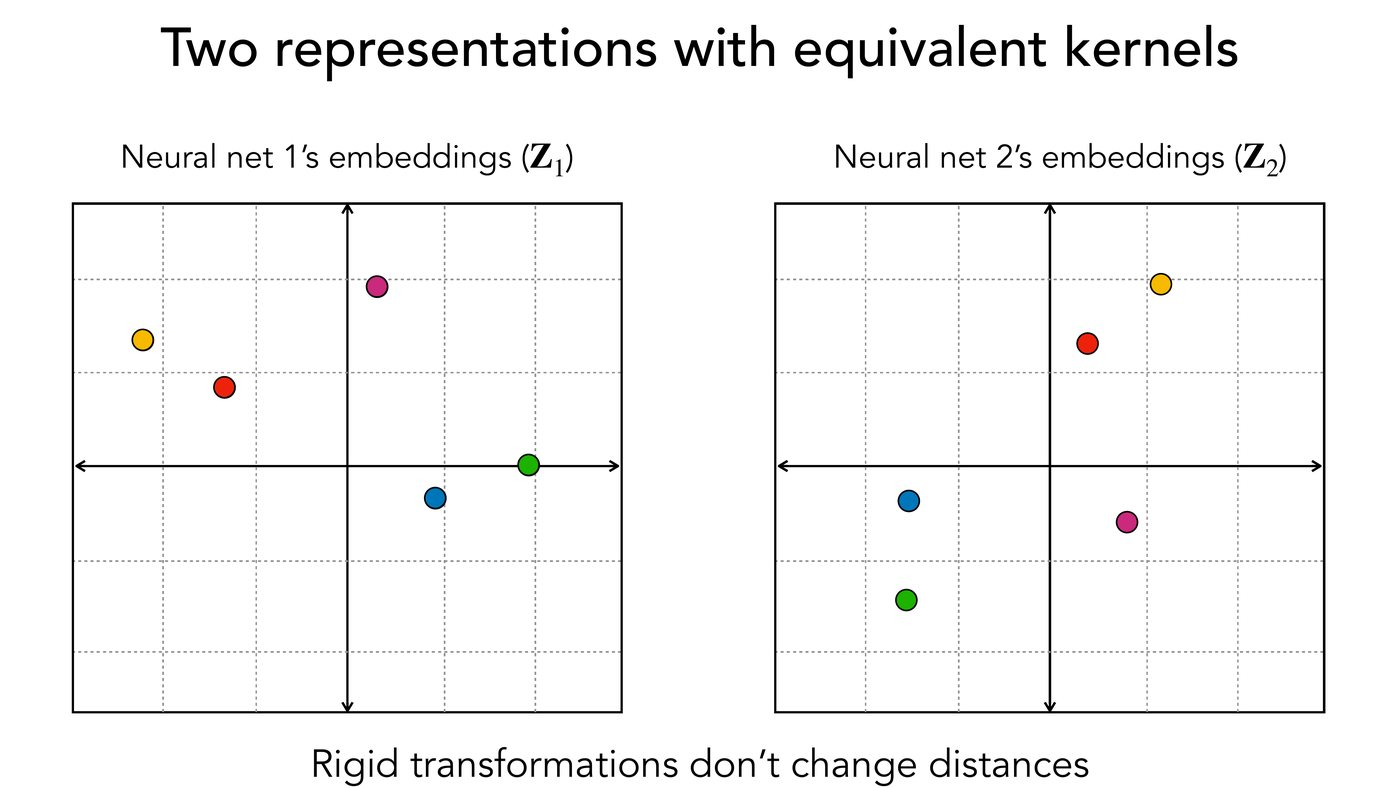
\includegraphics[width=0.82\textwidth]{figures/representational-geometry-1.jpg}
\caption{The invariance Isola argues for, from the Representational Geometry lecture. The
two panels hold the same five points related by a rigid transformation: every coordinate
changes, no pairwise distance does. The kernels are therefore identical and the two networks
count as the same representation, whereas a coordinate-wise comparison sees two unrelated
clouds.}
\label{fig:representational-geometry-1}
\end{figure}

\begin{figure}[htbp]
\centering
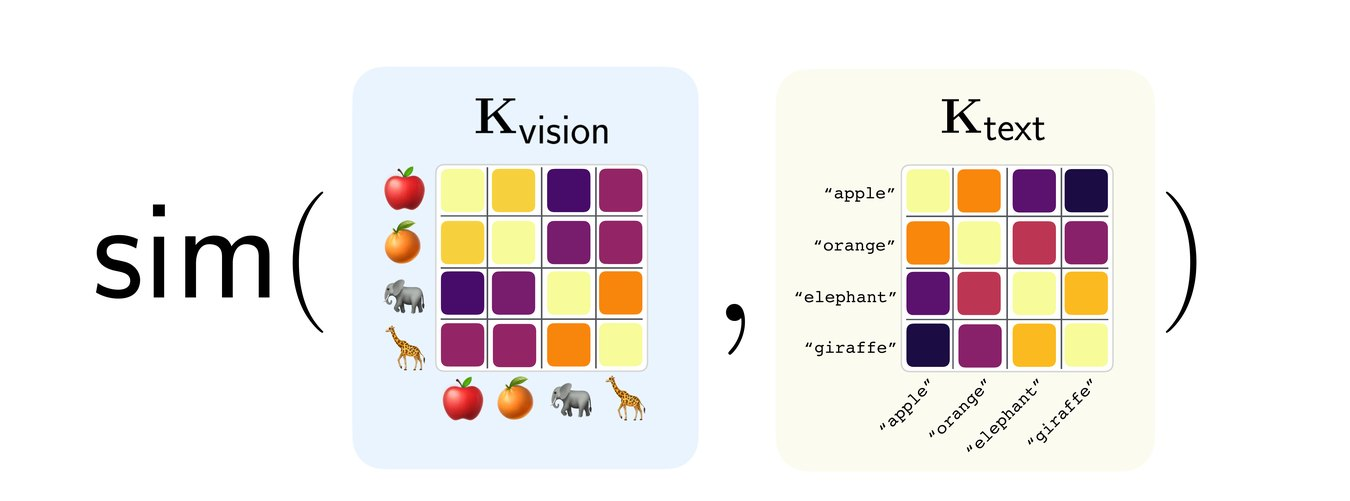
\includegraphics[width=0.86\textwidth]{figures/representational-geometry-2.jpg}
\caption{What cross-modal comparison actually compares, from the Representational Geometry
lecture. Each model is reduced to its own kernel matrix over the same four concepts, one from
images and one from the words naming them, and the two matrices are then compared. Nothing
requires the embeddings to share a dimension or a basis, only that both induce distances over
the same items.}
\label{fig:representational-geometry-2}
\end{figure}

\paragraph{Convergence, measured against humans and across modalities.} With a metric fixed,
the empirical section asks which representations actually agree. Against human similarity
judgements collected in DreamSim~\citep{fu2023}, DINO~\citep{caron2021} came out closest,
which is notable because DINO is trained on no human judgements at all. The same machinery,
borrowed from representational similarity analysis in neuroscience~\citep{kriegeskorte2008,
yamins2014}, then compares a vision model to a language model by asking whether their kernels
are alike (Figure~\ref{fig:representational-geometry-2}). The reported answer is that stronger
models converge, and that alignment increases with scale and over
time~\citep{huh2024}, which is the trend in
Figure~\ref{fig:representational-geometry-3}.\footnote{The personal notes add a caveat absent from the
slides, that open-source LLMs ``hasn't really increased though''. Recorded as a contemporaneous
observation, not as a lecture claim.} The lecture refuses to leave ``same'' vague and
offers three hypotheses: convergence to the same embedding vectors (identity), to the same
global kernel (glocal isometry), or to the same local neighbourhoods and clusters (local
ordinal isometry). Two theoretical results are sketched. A contrastive learner with an NCE
objective converges to pointwise mutual information,
\[
  \inner{\rep(\xin_a)}{\rep(\xin_b)} \;\approx\;
  \log \frac{P_{\text{co}}(\xin_a, \xin_b)}
            {P_{\text{co}}(\xin_a)\,P_{\text{co}}(\xin_b)},
\]
\noindent so for bijective discrete observation functions the PMI over observations equals
the PMI over underlying events, which forces different modalities onto the same kernel.
Separately, two CLIP-like models are claimed to converge to representations related by an
orthogonal transform $\mat{Q}$~\citep{gupta2026}.

\begin{figure}[htbp]
\centering
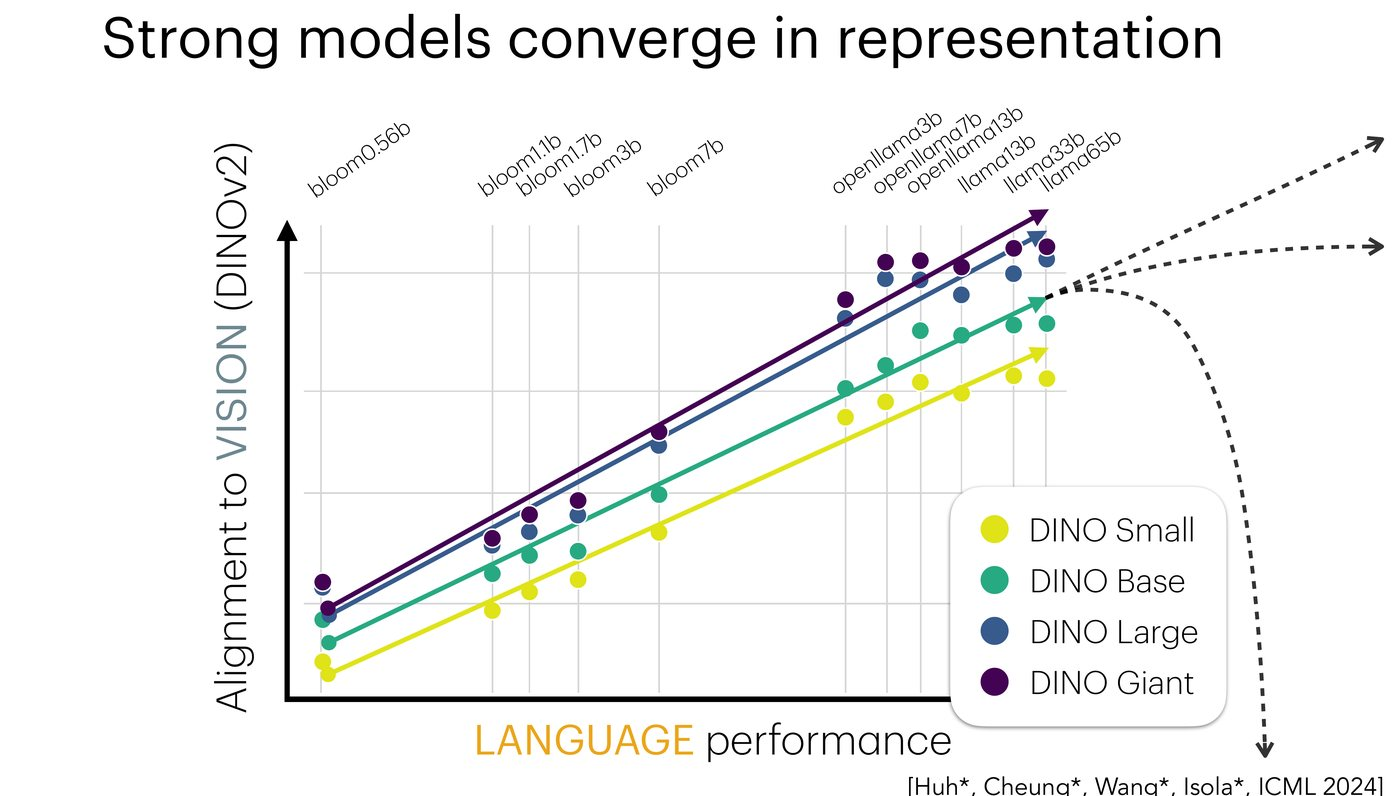
\includegraphics[width=0.84\textwidth]{figures/representational-geometry-3.jpg}
\caption{The central empirical claim of the Representational Geometry lecture. Alignment of a
language model's kernel to a vision model's (DINOv2) rises with the language model's own
performance, across the BLOOM and LLaMA families and across four DINO sizes. Better language
models look more like vision models, without ever having seen an image.}
\label{fig:representational-geometry-3}
\end{figure}

\paragraph{Alignment as a target, and what it costs.} If models converge anyway, alignment can
be engineered. Aligned representations let models share supervision and data, and a common
representation is a bridge for translation. The striking part is that paired data is not
required: vec2vec translates between embedding spaces using a GAN with a cycle-consistency
loss and a kernel-matching loss~\citep{jha2025}, an idea with a direct ancestor in
unsupervised word translation~\citep{conneau2018}, while REPA aligns a generative model's
representation to a pretrained one~\citep{yu2024}. Isola then lists the detriments without
softening them: alignment reduces diversity in the population of models; where one modality
has access to qualitatively different information, alignment destroys exactly that
information; and there may be no single best representation for all problems, which he notes
is not merely a practical worry but true in theory.

\section*{Notation}

$\rep$ and $\repB$ denote representations, $z = \rep(\xin)$ an embedding, $Z$ a point cloud
over a dataset, $h$ a map fitted between two embeddings, $\kernel$ a kernel matrix and $\Hcent$ the
centring matrix. One clash to
watch: $\Hcent$ here is a centring matrix, whereas
Chapter~\ref{ch:10-efficient-learning} uses $\Hess$ for a Hessian. Both follow their speaker's
usage and are kept visually distinct throughout.

\section*{Why it matters}

This is the lecture the personal notes cover in most detail, and it connects outward more than any
other. The claim that distance is the only thing worth preserving is the same
instinct that drives geometric deep learning
(Chapter~\ref{ch:11-geometric-deep-learning}), where invariance is imposed by construction
rather than measured after the fact. The convergence story is a counterpoint to Cho on
estimation (Chapter~\ref{ch:05-statistics-estimation}): Isola measures agreement between two
learned objects, Cho asks whether a learned estimator is even unbiased. And the tension
between alignment and diversity bears directly on CLIP's contrastive objective, which the summer
school's multimodal tutorial builds from scratch, since that loss is precisely the mechanism the
theory here predicts will drive convergence.

\begin{aside}
Isola's stronger claim, recorded in the personal notes rather than on the slides, is that
there is ``no future for distance functions that are not learned''. That sits in tension with
the argument of the lecture, which uses fixed metrics such as CKA to establish convergence.
If the yardstick is itself fitted to the objects being measured, the finding that models
converge becomes harder to state without circularity. Worth settling before leaning on
either claim.
\end{aside}

\chapter{Diffusion Models}
\label{ch:03-diffusion-models}

\lecturemeta{Sander Dieleman}{Google DeepMind}

Diffusion is one of two ways to break generation into easy steps, and almost every design
decision people argue about turns out to be downstream of a single equation for the forward
corruption process. Once
$\xt = \alpha(t)\xz + \sigma(t)\eps$ is on the board, the variance-preserving,
variance-exploding and flow-matching families are three choices of $\alpha$; predicting
$\xz$, $\eps$ or a velocity are interconvertible parameterisations of one object; guidance
is Bayes' rule applied to the score; and the question of why diffusion works so well on
images has a spectral answer that Dieleman states as a slogan. The final third is about
where the framework strains: distillation, discrete data, and what a latent space is for.

\section*{Key ideas}

\paragraph{Two roads to iterative refinement, and the space matters more than the road.}
Iterative refinement breaks the generative procedure into simpler steps in which all steps
are of comparable difficulty. Autoregression does this with the chain rule of probability,
$p(\xin) = \prod_i p(\xin_i \given \xin_{<i})$, and Dieleman's historical sequence makes the
point that the interesting variation was never the factorisation but the space it acts on:
pixels in PixelRNN and PixelCNN~\citep{oord2016pixelrnn}, raw amplitudes in
WaveNet~\citep{oord2016wavenet}, discrete latents in VQ-VAE~\citep{oord2017vqvae}. Diffusion
factorises differently, by iterative denoising, and the same lesson applies: production
systems run diffusion in a latent space, not in pixels, compressing a $3 \times 256 \times
256$ image to something like $8 \times 32 \times 32$ before the diffusion model ever sees
it.\footnote{This is the point the personal notes flag as ``Diffusion is done in latent
space, not in pixel space!''. The deck supports it with a pixels-versus-latents slide and a
pointer to regularising the latent space for generative modelling.}

\begin{figure}[htbp]
\centering
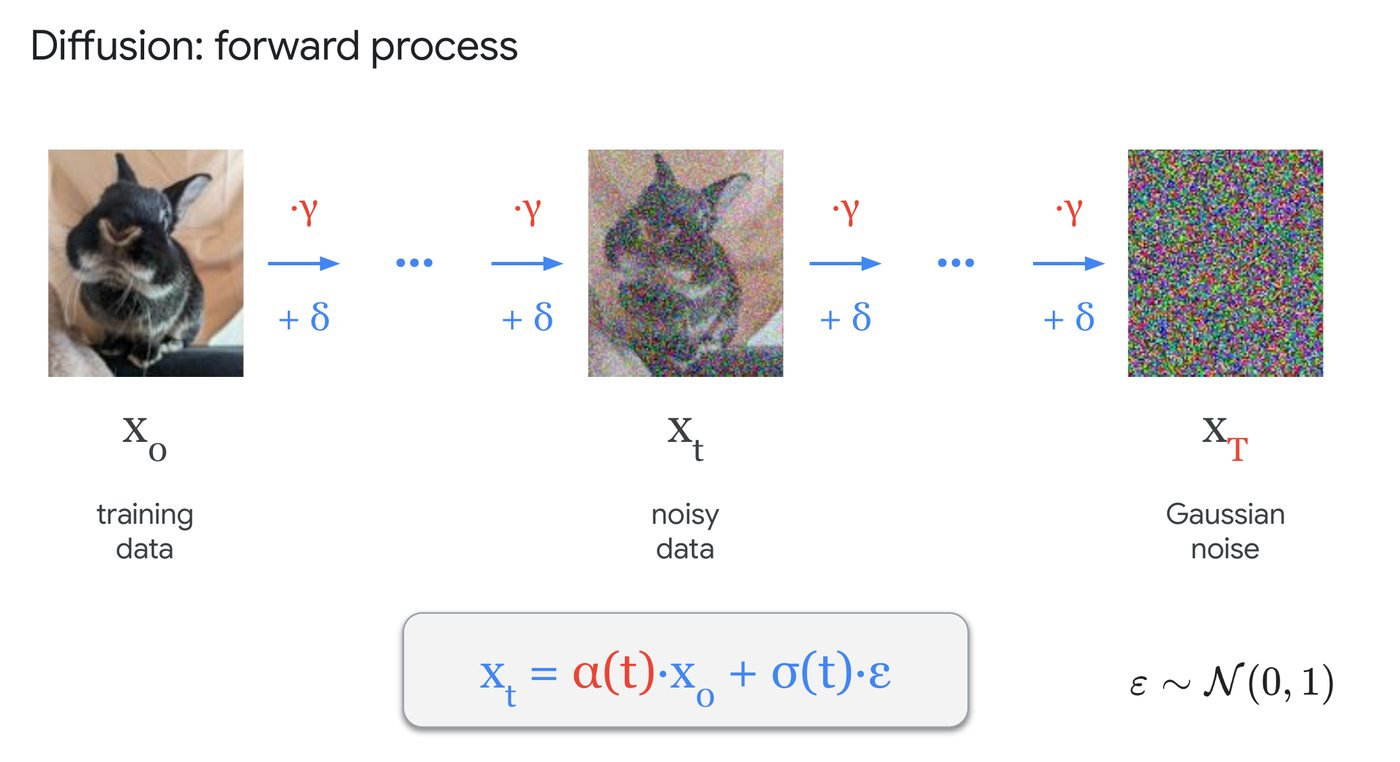
\includegraphics[width=0.82\textwidth]{figures/diffusion-models-1.jpg}
\caption{The forward process, from the Diffusion Models lecture. Each step scales by
$\gamma$ and adds noise $\delta$, carrying training data $\xz$ through noisy data $\xt$ to
pure Gaussian noise $\vect{x}_T$. The whole chain collapses to the boxed line,
$\xt = \alpha(t)\xz + \sigma(t)\eps$: corruption is just an interpolation between the data
and a sample of noise.}
\label{fig:diffusion-models-1}
\end{figure}

\paragraph{One equation for the forward process.} Corruption interpolates between data and
noise (Figure~\ref{fig:diffusion-models-1}),
\[
  \xt = \alpha(t)\,\xz + \sigma(t)\,\eps,
  \qquad \eps \dist \Normal(\vect{0}, \id),
\]
\noindent where $\sigma(t)$ is the noise schedule controlling the rate of corruption. The
families differ only in $\alpha$: variance-preserving takes
$\alpha = \sqrt{1 - \sigma^2}$, variance-exploding takes $\alpha = 1$, and rectified flow or
flow matching takes $\alpha = 1 - \sigma$. Presented this way, a literature that usually reads as three
separate methods collapses into one line with a parameter.

\paragraph{What the network predicts is a free choice.} Since $\xt$ is a linear combination
of $\xz$ and $\eps$, a prediction of one converts into a prediction of the other, so
$\xz$-prediction, $\eps$-prediction, $v$-prediction with
$v = \alpha(t)\eps - \sigma(t)\xz$~\citep{salimans2022}, and the flow-matching target
$\eps - \xz$~\citep{lipman2022} are reparameterisations rather than different models. The
same object appears again as the score $\grad_{\xin} \log p(\xin)$, which points toward
regions of high density, so knowing the gradient is knowing
$p$~\citep{hyvarinen2005, vincent2011}. In practice all of these are trained by minimising a
mean squared error.

\paragraph{Guidance is Bayes' rule, twice.} Dieleman's own phrase, and the one the personal notes
record, is that guidance is ``a cheat code'': it buys sample quality at the cost of
diversity. Classifier guidance is derived on the slide straight from Bayes' rule, in three
lines:
\[
\begin{aligned}
  p(\xin \given c) &\propto p(c \given \xin)\, p(\xin), \\
  \log p(\xin \given c) &= \log p(c \given \xin) + \log p(\xin) + C, \\
  \underbrace{\grad_{\xin} \log p(\xin \given c)}_{\text{conditional score}}
    &= \underbrace{\grad_{\xin} \log p(c \given \xin)}_{\text{classifier gradient}}
     + \underbrace{\grad_{\xin} \log p(\xin)}_{\text{unconditional score}}.
\end{aligned}
\]
\noindent The normalising constant differentiates away, which is the whole trick: the
conditional score is the unconditional score plus a classifier gradient, so an unconditional
model becomes conditional without retraining. A
scale factor $\guide$ on the second term acts as an inverse temperature, and the lecture is
careful about what it sharpens: it sharpens $p(c \given \xin)$, which is not the same thing
as sharpening $p(\xin)$ or $p(\xin \given c)$. Classifier-free guidance drops the separate
classifier: predict $\est{\xz}$ and $\est{\xz}_{|c}$ from one model trained with conditioning
dropout, take the difference $\delta$, and amplify it by $\guide$. The insight is that
$\delta$ is itself a Bayesian classifier, so this is Bayes' rule applied twice, and it is
less prone to adversarial examples than guiding with a real
classifier~\citep{nichol2022glide}. Figure~\ref{fig:diffusion-models-2} shows guidance as a geometric
operation on one sampling step, not a change to the model.

\begin{figure}[htbp]
\centering
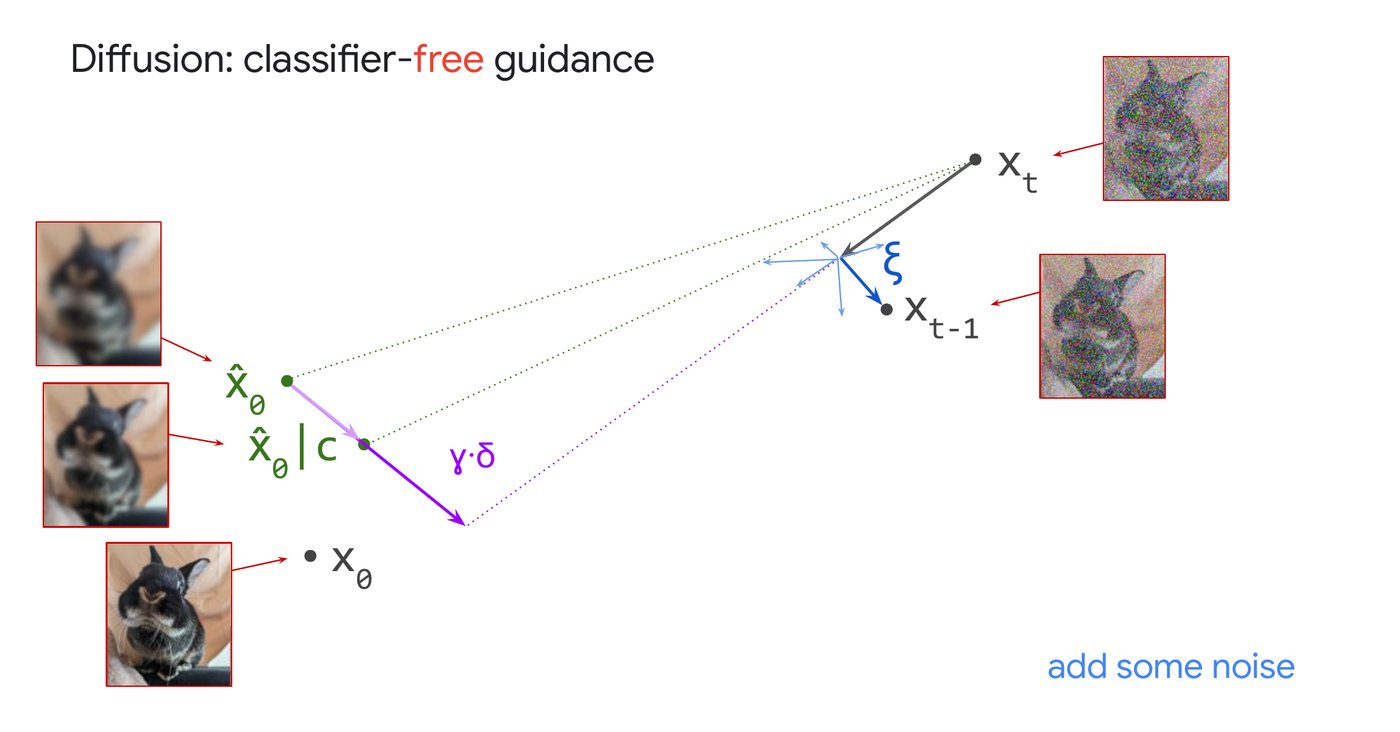
\includegraphics[width=0.86\textwidth]{figures/diffusion-models-2.jpg}
\caption{Classifier-free guidance as one sampling step, from the Diffusion Models lecture.
From the noisy state $\xt$ the model predicts both an unconditional $\est{\xz}$ and a
conditional $\est{\xz}_{|c}$; their difference $\delta$ is scaled by $\gamma$ and
extrapolated past the conditional prediction, then a small step is taken toward that
extrapolated target and fresh noise $\xi$ is added to reach $\vect{x}_{t-1}$. Note that the
guided target overshoots $\xz$ entirely, which is exactly why guidance trades diversity for
apparent quality.}
\label{fig:diffusion-models-2}
\end{figure}

\paragraph{Diffusion is approximate spectral autoregression.} The lecture's answer to why
diffusion works so well on images is spectral, and it is the insight the personal notes single out.
Natural images have a power spectrum that falls off steeply with spatial frequency, while
Gaussian noise is flat. Adding noise at level $\sigma$ therefore does not damage all scales
equally: it drowns everything above the frequency where the flat noise floor crosses the
image's decaying spectrum, and leaves the low frequencies almost intact
(Figure~\ref{fig:diffusion-models-3}). Sampling, run backwards, is then recovering
frequency bands roughly coarsest-first, which is why Dieleman puts it as diffusion being
approximate spectral autoregression~\citep{dieleman2023perspectives}. It also explains why
the trick transfers poorly to data without a decaying spectrum.

\begin{figure}[htbp]
\centering
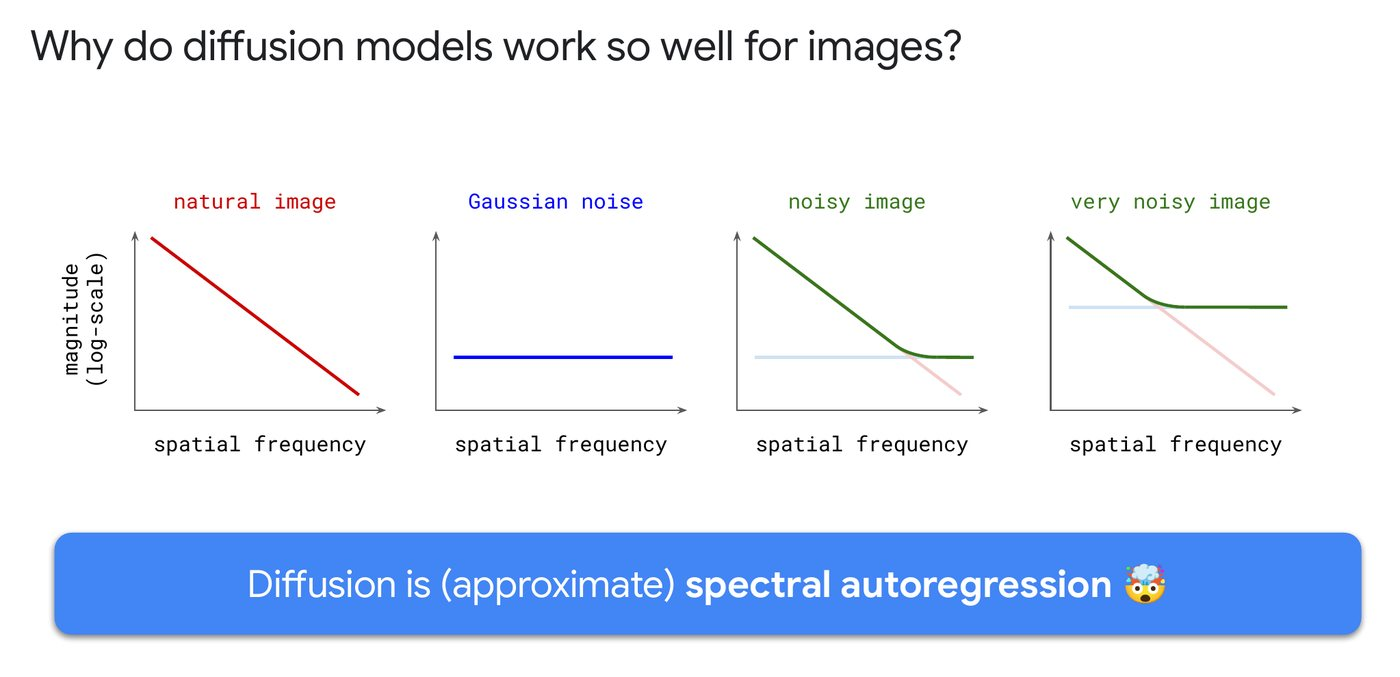
\includegraphics[width=0.88\textwidth]{figures/diffusion-models-3.jpg}
\caption{The spectral argument, from the Diffusion Models lecture. A natural image's
magnitude spectrum falls steeply with spatial frequency while Gaussian noise is flat, so
their sum is the pointwise maximum: at moderate noise the high frequencies are already
replaced by the noise floor, and at high noise only the lowest frequencies survive. Read
right to left, sampling restores frequency bands coarsest-first, which is the sense in which
diffusion is approximate spectral autoregression.}
\label{fig:diffusion-models-3}
\end{figure}

\paragraph{Where the framework strains.} Three limitations close the lecture.
Distillation into fewer sampling steps requires cutting corners, and the corners are entropy
and diversity first, then visual fidelity~\citep{dieleman2024paradox, song2023consistency}.
Discrete data breaks the score outright, since $\grad_{\xin} \log p(\xin)$ is undefined when
$\xin$ is discrete; the two escapes are to define a discrete corruption process, or to embed
the data in a continuous space, which is what CDCD does while deliberately making diffusion
look familiar to language-model practitioners by using an unmasked Transformer and a
cross-entropy loss instead of an MSE~\citep{dieleman2022cdcd}. And data curation is named as
essential for high-quality results while being structurally disincentivised in the research
community.

\section*{Notation}

$\xz$ is clean data, $\xt$ the corrupted state at time $t$, $\eps$ standard Gaussian noise,
$\alpha(t)$ and $\sigma(t)$ the interpolation coefficients, and $\guide$ the guidance scale.
The deck writes the guidance scale as a Greek gamma. It is $\guide$ here, to keep it clear of the
discount factor in Chapter~\ref{ch:04-intro-reinforcement-learning}.

\section*{Why it matters}

The parameterisation argument travels furthest. Whenever a literature presents $n$ competing
methods, ask whether they are $n$ choices of one coefficient.
The spectral analysis connects directly to Stanković's lecture
(Chapter~\ref{ch:09-spectral-analysis-dags}), which also treats a spectrum as the object to
manipulate, though on graphs rather than grids, and to Veličković's argument
(Chapter~\ref{ch:11-geometric-deep-learning}) that the structure of the data domain should
dictate the model. Classifier-free guidance reappears in the summer school's
multimodal tutorial, where it is the single line the notebook asks to be written by hand.

\begin{aside}
Two threads to pull. The personal notes record the claim that diffusion models are
essentially RNNs, which permits training much deeper networks. That framing is not on the
slides in those words, though it is consistent with the iterative-refinement picture where
one network is applied repeatedly with a time input; treat it as a remark from the room
rather than a slide. Second, the deck's closing list of untouched topics includes flow maps,
also flagged in the personal notes, pointing at Dieleman's blog~\citep{dieleman2026flowmaps}. That
is the natural continuation of the unification of diffusion and flow matching set out above.
\end{aside}

\chapter{Introduction to Reinforcement Learning}
\label{ch:04-intro-reinforcement-learning}

\lecturemeta{Andreea Deac}{Isomorphic Labs}

The lecture is built on one identity used three ways. Bellman's equation,
$\Vf^{\pi}(s) = \Ex[\rt + \disc \Vf^{\pi}(s')]$, admits a full-expectation backup, a
one-step bootstrapped backup and a full-depth sampled backup, and dynamic programming,
temporal difference learning and Monte Carlo are exactly those three choices. Everything
else in the lecture is either what goes wrong in the absence of that identity, namely
REINFORCE's inability to assign credit to individual actions, or what has to be bolted on
afterwards to make policy gradients survive contact with their own data. The last section
lands on GRPO and RLVR, and the framing is that the modern LLM stack is this material with a
verifiable reward substituted for a learned one. Deac also ran the talk as a live bandit,
and reported that it failed.

\section*{Key ideas}

\paragraph{The problem is defined by where the data comes from.} Four contrasts with
supervised learning organise the setup: the data is self-induced by acting rather than a
fixed i.i.d.\ set of pairs, the signal is a reward rather than a correct label, feedback may
arrive many steps later rather than immediately, and the goal is to act so as to maximise
long-term return rather than to learn a map. Formally an MDP is
$(\States, \Actions, \Trans, \Rew, \disc)$ with $\Trans(s' \given s, a)$ and
$\Rew(s,a) = r$, the Markov property meaning the future depends on the present state alone.
A policy $\pi(a \given s)$ produces a trajectory
$\traj = (s_0, a_0, r_0, s_1, \dots)$ scored by the return
$\ret_t = \sum_{k \ge 0} \disc^{k} r_{t+k}$, and the objective is
$\obj(\params) = \Ex_{\traj \dist \pol}[\ret(\traj)]$. The deck's own reference slide points
at Sutton and Barto for all of this~\citep{sutton2018}.

The motivation for $\disc$ is the best in the whole set of lectures because it is
arithmetic rather than assertion. Three gridworld trajectories score 99, 100 and 101
undiscounted, so the greedy detour wins and nothing prevents the agent cycling through a
$+100$ cell forever. At $\disc = 0.95$ the same three trajectories, of length 3, 7 and 9
steps, score 89.2, 73.5 and 67.1: the short path now wins, and the infinite loop sums to
about 10 rather than diverging.

\paragraph{Policy gradients, and the credit they cannot assign.} The direct approach is
gradient ascent on $\obj$, but $\params$ sits in the sampling distribution rather than in the
return, so differentiating through $\ret$ after sampling gives zero and the trajectories
cannot be enumerated. The log-derivative trick moves the gradient inside the expectation,
\[
  \grad_{\params} \Ex[f] = \sum_{\traj} f \grad_{\params} p
  = \sum_{\traj} f \frac{\grad_{\params} p}{p} p
  = \Ex\bigl[f \grad_{\params} \log p\bigr],
\]
\noindent which yields the policy gradient theorem,
$\grad_{\params}\obj = \Ex_{\traj}\bigl[\sum_t \grad_{\params} \log \pol(\at \given \st)
\ret_t\bigr]$: push up the log-probability of actions in proportion to how good the outcome
was, and never differentiate through the environment. The lecture then immediately shows the
cost of that convenience (Figure~\ref{fig:intro-reinforcement-learning-2}). Credit attaches
to whole action sequences, so 58 of 104 genuinely bad actions were pushed up simply because
the episode they belonged to went well.

\begin{figure}[htbp]
\centering
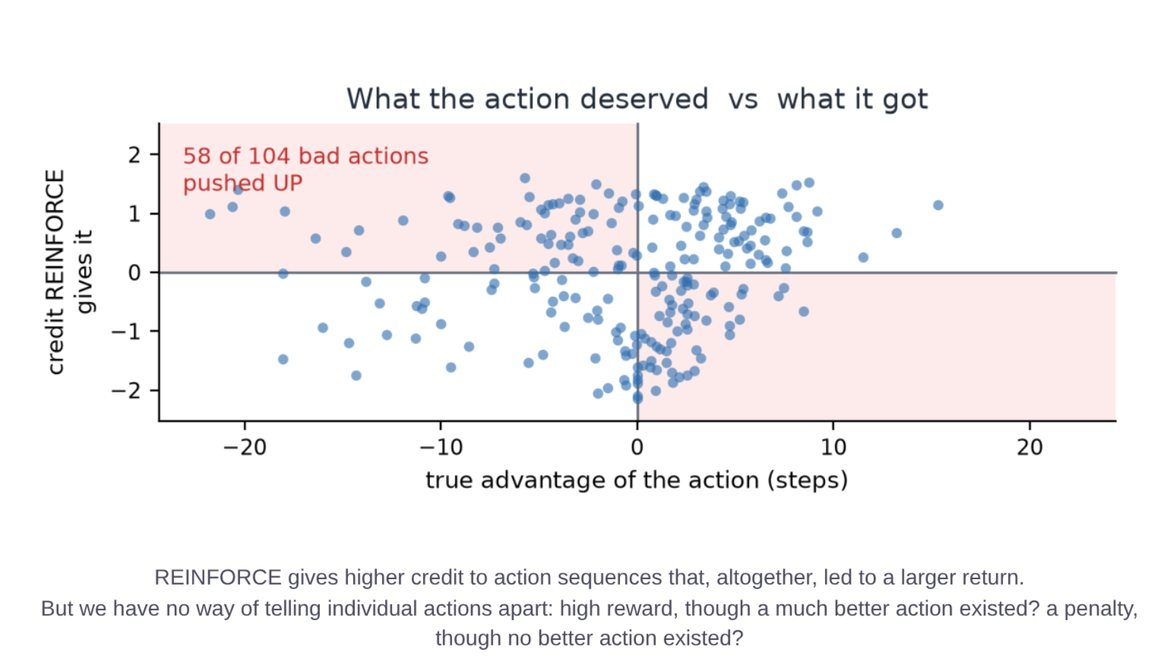
\includegraphics[width=0.62\textwidth]{figures/intro-reinforcement-learning-2.jpg}
\caption{Why REINFORCE needs a baseline, from the Introduction to Reinforcement Learning
lecture. Each point is one action, with its true advantage on the horizontal axis and the
credit REINFORCE assigned on the vertical. The shaded quadrants are the mistakes: actions
that hurt but were reinforced, and actions that helped but were penalised. The lecture's
count is 58 of 104 bad actions pushed up.}
\label{fig:intro-reinforcement-learning-2}
\end{figure}

\paragraph{One Bellman equation, three backups.} Value functions supply the missing notion
of what to expect. Writing Bellman's equation out,
\[
  \Vf^{\pi}(s) = \Ex\bigl[r + \disc \Vf^{\pi}(s')\bigr]
   = \sum_{a} \pi(a \given s) \sum_{s'} \Trans(s' \given s, a)
     \bigl[r + \disc \Vf^{\pi}(s')\bigr],
\]
\noindent the recursion $\ret = r + \disc \ret'$ is what lets the problem be solved
backwards, illustrated with a Montenegrin road map: if the best route from Podgorica to Kotor
passes through Cetinje, the best route from Cetinje to Kotor is part of it. The three ways to
use it (Figure~\ref{fig:intro-reinforcement-learning-1}) are dynamic programming, taking the
full expectation and needing the model $\Trans$; temporal difference,
$\Vf(s) \leftarrow \Vf(s) + \alpha[r + \disc \Vf(s') - \Vf(s)]$, one sampled step
bootstrapped off its own estimate; and Monte Carlo,
$\Vf(s) \leftarrow \Vf(s) + \alpha[\ret_t - \Vf(s)]$, one sample to termination. Monte Carlo
is unbiased with high variance; TD reverses the trade, taking bias from the Markov assumption
and from trusting its own current estimates. An eight-episode exercise makes the difference
concrete: with $\Vf(B) = 6/8$, batch Monte Carlo puts $\Vf(A) = 0$ because the one episode
through $A$ returned 0, while batch TD puts $\Vf(A) = 0.75$ because the transitions imply $A$
leads to $B$ with certainty. Monte Carlo fits the observed data, TD fits the MDP that the data
implies.

\begin{figure}[htbp]
\centering
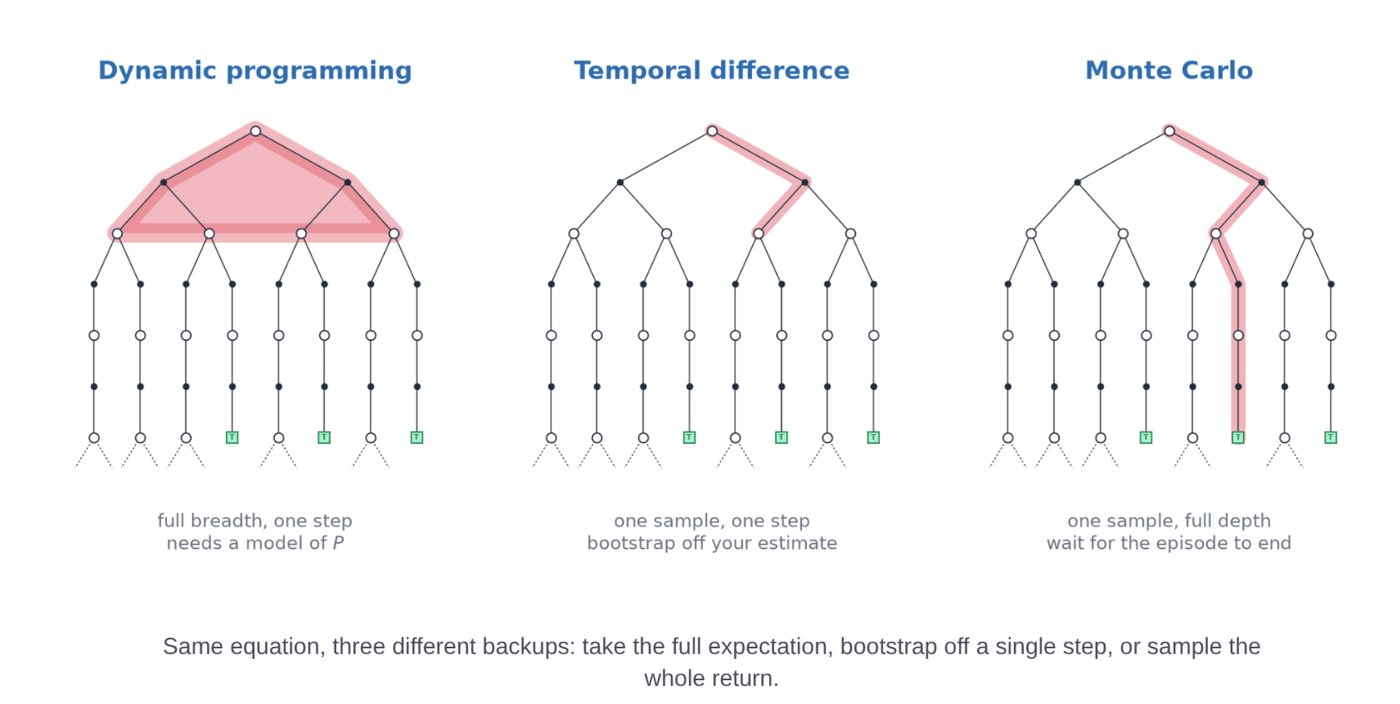
\includegraphics[width=0.82\textwidth]{figures/intro-reinforcement-learning-1.jpg}
\caption{The organising figure of the Introduction to Reinforcement Learning lecture, titled
``Three ways to use Bellman''. Shading marks which part of the tree each backup consults:
dynamic programming sweeps one step in full breadth, temporal difference follows a single
sampled step and then bootstraps, Monte Carlo follows one sampled path to a terminal state.
The equation is the same in all three cases.}
\label{fig:intro-reinforcement-learning-1}
\end{figure}

\paragraph{Making policy gradients survive their own data.} Subtracting a baseline $b(s)$
leaves the gradient unbiased, since
$\sum_a b(s) \grad_{\params} \pol(a \given s) = b(s)\grad_{\params} 1 = 0$, and reduces
variance; using $\Vf$ as the baseline gives the advantage
$\Adv(s,a) = \Qf(s,a) - \Vf(s)$, which also puts states with different reward scales on a
common footing. Actor-critic learns both, and generalised advantage estimation reintroduces
the $n$-step bias-variance dial,
$\Adv_t^{\text{GAE}} = \sum_{k \ge 0} (\disc \lambda)^{k}
 [r_{t+k} + \disc \Vf(s_{t+k+1}) - \Vf(s_{t+k})]$, with $\lambda = 0$ high bias and
$\lambda = 1$ low bias. Two failure modes follow. Premature collapse is met with entropy
regularisation, $\params \leftarrow \params + \lr \grad_{\params}(\obj(\params)
+ \beta H(\pol))$, annealing $\beta$ down. Instability is worse: the data comes from the
current policy, so one oversized update breaks behaviour and the next batch is collected by
the broken policy, a negative spiral. TRPO constrains it,
$\max_{\params} \Ex[(\pol / \pi_{\text{old}})\Adv]$ subject to
$\KL{\pi_{\text{old}}}{\pol} \le \delta$, at the price of a second-order solve; PPO clips the
ratio instead for the same effect with first-order optimisation.

\paragraph{Where this lands in 2026.} The reward changes character: RLHF's learned model of
human preference gives way to RLVR's verifiable checker, does the test pass, is the answer
right, which is cheaper, harder to hack and scalable~\citep{lambert2024tulu3}.
DeepSeek-R1~\citep{deepseek2025r1} is presented as evidence that RL on a base model with no
supervised finetuning can elicit reasoning and self-correction. GRPO~\citep{shao2024grpo} is
called ``the one algorithm to teach'': PPO must carry a critic typically the size of the
policy, whereas GRPO samples a group of answers per prompt and standardises within the group,
$\Adv_i = (r_i - \text{mean})/\text{std}$, with no critic network at all. Genie
3~\citep{bruce2024genie} is contrasted with dynamic programming: where DP needs an explicit
$\Trans$, Genie learns implicit dynamics from data and generates interactive future states
from text, so environments themselves become generatable.

\section*{Notation}

$\States, \Actions, \Trans, \Rew, \disc$ for the MDP, $\pi$ for a policy, $\traj$ for a
trajectory, $\ret_t$ for the return, $\Vf$ and $\Qf$ for state and action values, $\Adv$ for
the advantage, $\alpha$ for the value-update step size and $\lr$ for the policy step size.
Here $\disc$ is unambiguously the discount factor, unlike the same Greek letter used for the
guidance scale in Chapter~\ref{ch:03-diffusion-models}.

\section*{Why it matters}

This chapter is the prerequisite for the summer school's
reinforcement learning tutorial, which implements REINFORCE, PPO and GRPO in that order and so
retraces this argument in code. The i.i.d.\ discussion around experience
replay is the same concern Chandar closed on
(Chapter~\ref{ch:01-intro-deep-learning}) and that Lyle and Pascanu develop
(Chapters~\ref{ch:06-continual-learning} and~\ref{ch:07-to-be-figured-out}): replay exists
because SGD assumes independent samples and consecutive transitions are not independent,
which is continual learning's problem solved by brute force.

\begin{aside}
The most useful thing in this lecture is not on a slide about RL at all. Deac turned the
talk into a nine-armed bandit over slide layouts and background colours, with audience votes
as reward, and then reported the outcome honestly: 53 rounds, 0 votes, every round skipped.
The closing slide lists why real-world RL is hard using her own failure as the example:
reward confounded with content, non-stationarity as the audience tires, sparse and noisy
feedback, varying turnout, delayed and batched rewards, and an assumption that the two
dimensions were independent when they were not. Any applied RL project should expect to fail
in at least two of those ways before it fails in an interesting one.
\end{aside}

\chapter{Statistics: Learning to Estimate}
\label{ch:05-statistics-estimation}

\lecturemeta{Kyunghyun Cho}{New York University}

Cho's lecture has one thesis, stated plainly two-thirds of the way through and worth quoting
because it reorganises a great deal of statistics: inference does not have to be about
inverting the generative process. The conventional route to any estimand is to model the data
generating distribution and then invert it, and the lecture's claim is that this step is
optional. Given the ability to sample problems with known answers, estimator design becomes a
supervised regression problem, and gradient descent finds an estimator that beats the textbook
one. The argument is built on a deliberately trivial example, the population standard
deviation, then repeated for mutual information, Bayesian predictive distributions and causal
effects, and finally turned back on theory to redefine what identifiability means.

\section*{Key ideas}

\paragraph{Start with something embarrassingly simple.} The sample standard deviation is a
biased estimate of the population standard deviation, because the square root sits outside
the expectation. Rather than deriving a correction, Cho asks why estimator design is not
simply a minimisation problem. Given pairs $(\mathcal{D}, \params)$ of a sample set and the
true population standard deviation, a good estimator $F$ has low
$\MSE$, and the only source of variation is the sampling that produced $\mathcal{D}$. So
define a meta-distribution $P_\Gamma$ over distributions of known population standard
deviation and minimise over a hypothesis class $\mathcal{F}$ of estimators,
\[
  \min_{F \in \mathcal{F}} \;
  \Ex_{\pi \dist P_\Gamma}\Bigl[\,
    \Ex_{\mathcal{D} \dist \pi}\bigl[\,
      \MSE\bigl( F(\mathcal{D}),\, \mathrm{stdev}(\pi) \bigr)
    \bigr]
  \Bigr].
\]
\noindent As the slides note, this is exactly training a regression model: a data distribution
$P_\Gamma$, a set of samples as input, a real number as output, and an MSE loss.

\paragraph{The architecture is forced by an invariance.} An estimator over a sample set must
be permutation invariant, so $F$ is a transformer with the positional embeddings removed,
followed by aggregation, which the lecture calls Set
Transformer++~\citep{zhang2022setnorm}.\footnote{``Set Transformer++'' is the lecture's own name
for the architecture. The cited paper is on set norm and equivariant skip connections for deep
sets, and does not use that name.} This is a small but neat
instance of the geometric deep learning argument
(Chapter~\ref{ch:11-geometric-deep-learning}): the symmetry of the data dictates the
architecture, here without either speaker mentioning the other.

\paragraph{It works, and the reason it works is the interesting part.} The learned estimator
is essentially unbiased where \texttt{np.std} is not, is more sample-efficient, converges as
the sample size grows, and, importantly, works on log-normal distributions that were held out
of training (Figure~\ref{fig:statistics-estimation-1}). Cho's reading of that last fact is
the pivot of the lecture. Had the network been implicitly identifying the underlying
distribution, fitting it, and then correcting the sample standard deviation, it would fail on
a family it had never seen. It does not fail, so it is doing something else: bypassing
density estimation and going straight to inference. Supervised learning found a new estimator
of the population standard deviation.

\begin{figure}[htbp]
\centering
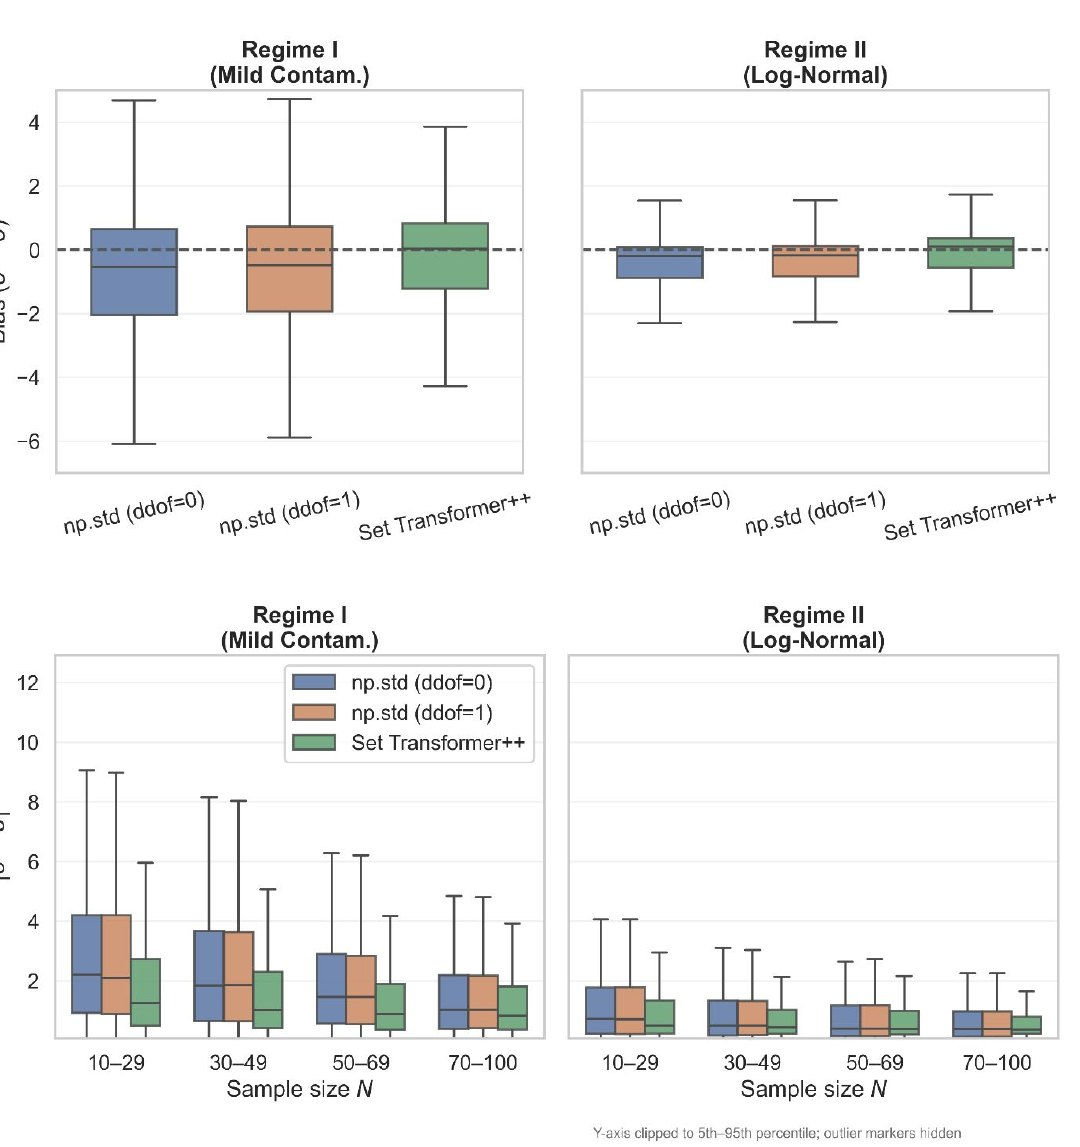
\includegraphics[width=0.60\textwidth]{figures/statistics-estimation-1.jpg}
\caption{The proof of concept from the Statistics lecture. Top, bias
$\est{\sigma} - \sigma$ for two \texttt{numpy} estimators and the learned one, under mild
contamination and under a log-normal regime that was held out of training. Bottom, absolute
error against sample size. The learned estimator is centred on zero where \texttt{np.std} sits
below it, and it holds up on the unseen family, which is the evidence that it is not
implicitly fitting a density.}
\label{fig:statistics-estimation-1}
\end{figure}

\paragraph{The same move, three more times.} Mutual information is defined through density
ratios, so the reflex is to estimate the ratio; MIST instead attends over both the sample
axis and the dimension axis and predicts MI directly, reportedly outperforming existing
estimators, keeping both bias and variance low, largely escaping the curse of dimensionality,
and generalising to dimensionalities and sample sizes outside its training range. Once available,
a learned estimator can itself serve as an objective function. The Bayesian predictive
distribution is defined through the posterior, so the reflex is to approximate the posterior;
prior-data fitted networks approximate the predictive distribution directly with a
transformer~\citep{muller2022pfn}, matching exact Gaussian-process predictions closely at a
fraction of the cost of MCMC. That raises the obvious objection, where did the prior go, and
the answer is to supply it in context: sample a prior, sample datasets from it, and train
multi-task in-context learning to condition on both. Causal effects get the same treatment
under the name black-box causal inference~\citep{bynum2025bbci}, recovering estimators for observed
confounders and for instrument variables, and tested on the LaLonde job-training
data~\citep{lalonde1986}. A
recurring caveat is that diversity of the training prior, not just its correctness,
determines how far the estimator generalises.

\paragraph{Computational identifiability.} The theoretical payoff is a redefinition.
Mathematical identifiability says that if two observations of infinitely many samples have
matching distributions then the parameters of interest must coincide. Cho proposes
\emph{computational} identifiability instead~\citep{bynum2026identifiability}, defined relative to
three operational constraints: a prior over the problem space, a hypothesis space, and an optimisation
algorithm. The procedure is explicit. Take a causal query; define a prior over structural
causal models combining given and simulated distributions; define a hypothesis space
reachable by the chosen optimiser; search for the best estimator; and if it is accurate for most of
the sampled SCMs, declare the query identifiable. Unlike the mathematical version this is
soft, so one can compute $p(\text{identifiable} \given \varepsilon)$ and plot it as a curve.

\section*{Notation}

$\params$ is the estimand, $\est{\params}$ or $F(\mathcal{D})$ the estimate, $\mathcal{D}$ a
sample set, $\pi$ a single data distribution and $P_\Gamma$ the meta-distribution over such
distributions. The distinction between $\pi$ as a distribution over data here and $\pi$ as a
policy in Chapter~\ref{ch:04-intro-reinforcement-learning} is the speakers' own; both are
standard in their fields and neither is changed.

\section*{Why it matters}

This is the most quietly radical lecture of the week, and it cuts against
Chapter~\ref{ch:02-representational-geometry} in a way worth noticing. Isola measures whether
learned representations agree, using fixed metrics as the yardstick; Cho's programme suggests
the yardstick itself should be learned, which is the same instinct as Isola's own remark that
there is no future for unlearned distance functions. Read together they point at a world where
both the model and the measurement are fitted, and where the burden shifts entirely onto the
prior over problems. The bias-variance material also connects to Alistarh's linearity theorem
(Chapter~\ref{ch:10-efficient-learning}), which is another attempt to predict an error rather
than measure it.

\begin{aside}
The load-bearing assumption is easy to miss because the examples are so clean. Every learned
estimator here is only as good as the meta-distribution $P_\Gamma$ it was trained over, and
for the standard-deviation example we can write that prior down honestly. For causal queries
we cannot, which is precisely why computational identifiability is defined relative to a
prior rather than absolutely. That makes it an honest notion, but it also means a query can
be declared identifiable under one prior and not another, and the lecture does not claim
otherwise.
\end{aside}

\chapter{Continual Learning}
\label{ch:06-continual-learning}

\lecturemeta{Clare Lyle}{Google DeepMind}

Lyle's framing is that continual learning is two problems, not one, and that standard
training is bad at both. A network must remember what it learned before, and it must remain
able to learn something new. The first failure is catastrophic forgetting and has been known
since the early 1990s; the second is loss of plasticity and is the subject of most of the
lecture, because it is both less obvious and better understood mechanistically. The line that
organises everything is slide 17, which reads: ``Continual learning doesn't have to be hard
(unless you want to use a neural network)''. The difficulties are properties of the optimiser and the
architecture, not of the problem statement, and once diagnosed that way most of them have
mundane fixes.

\section*{Key ideas}

\paragraph{Two problems and a meta-problem.} Problem one is remembering the
past~\citep{kirkpatrick2017}. Problem two is retaining plasticity, the capacity to keep
learning at all. The meta-problem is evaluation, and neither option is satisfactory: train on a pre-specified sequence of tasks, which is artificial, or find an
application that is naturally continual, which is uncontrolled. That tension sits under every result in the field.

\begin{figure}[htbp]
\centering
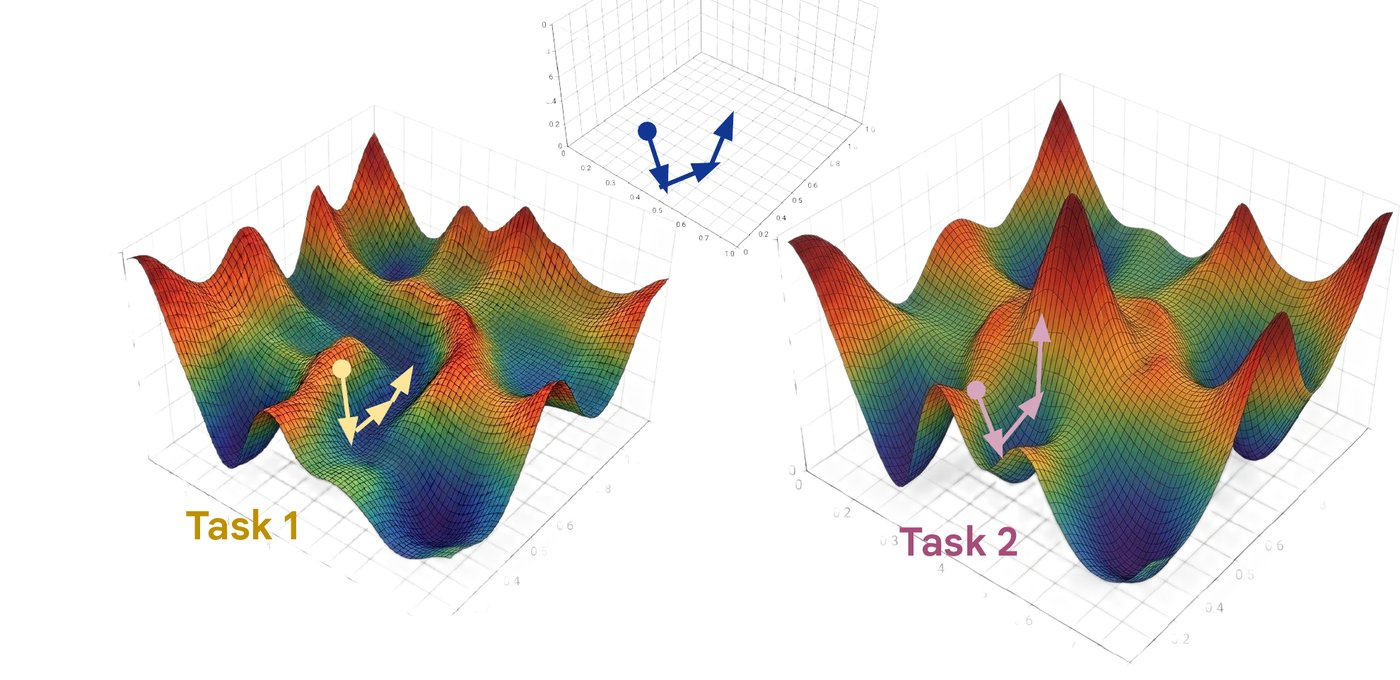
\includegraphics[width=0.88\textwidth]{figures/continual-learning-2.jpg}
\caption{The geometric intuition for catastrophic forgetting, from the Continual Learning
lecture. The same parameters sit on two different loss surfaces, one per task, and the descent
directions the two tasks ask for are not aligned, as the inset axes make explicit. A step that
lowers the task-two loss can climb the task-one loss, so progress on the new task is paid for
out of the old one.}
\label{fig:continual-learning-2}
\end{figure}

\paragraph{Forgetting is gradient conflict, and the fixes follow from that.} The intuition given is geometric
(Figure~\ref{fig:continual-learning-2}): gradients on different tasks often conflict, so a step
that helps task two moves parameters out of the region that solved task one. Three families of solution follow
directly from the diagnosis, and the lecture states them in plain terms before naming any
method. Do not change the parameters used for the old task too much, which is regularisation
and, with a different mechanism, sparsity and network expansion. Keep the old data around and
keep training on it, which is replay. Or periodically reset the model and retrain on
everything, which pairs with distillation. Lyle's practical verdict appears again in the summary: if the data can be kept, the first problem is easy. Only under a memory constraint
does it require finesse.

\paragraph{Loss of plasticity has a mechanism, and it is the optimiser.} Under repeated task
changes networks become less trainable over time, in the extreme case with dead
ReLUs and a model emitting a uniform distribution. Two causes are separated. First, gradual
convergence toward bad parameters, diagnosed through the empirical NTK matrix at convergence.
Second, and more surprising, destructive updates that happen almost immediately after a task
change. The reason is that optimisers are built for stationary problems. In Adam the second
moment estimate decays slowly, with the usual 0.99, so it reflects the small gradients seen at
the end of the previous task; when the loss changes the numerator grows at once while the
denominator lags, and the effective step size becomes enormous
(Figure~\ref{fig:continual-learning-1}). The loss landscape has meanwhile evolved to be stable
only at the small step size it was trained with.

\begin{figure}[htbp]
\centering
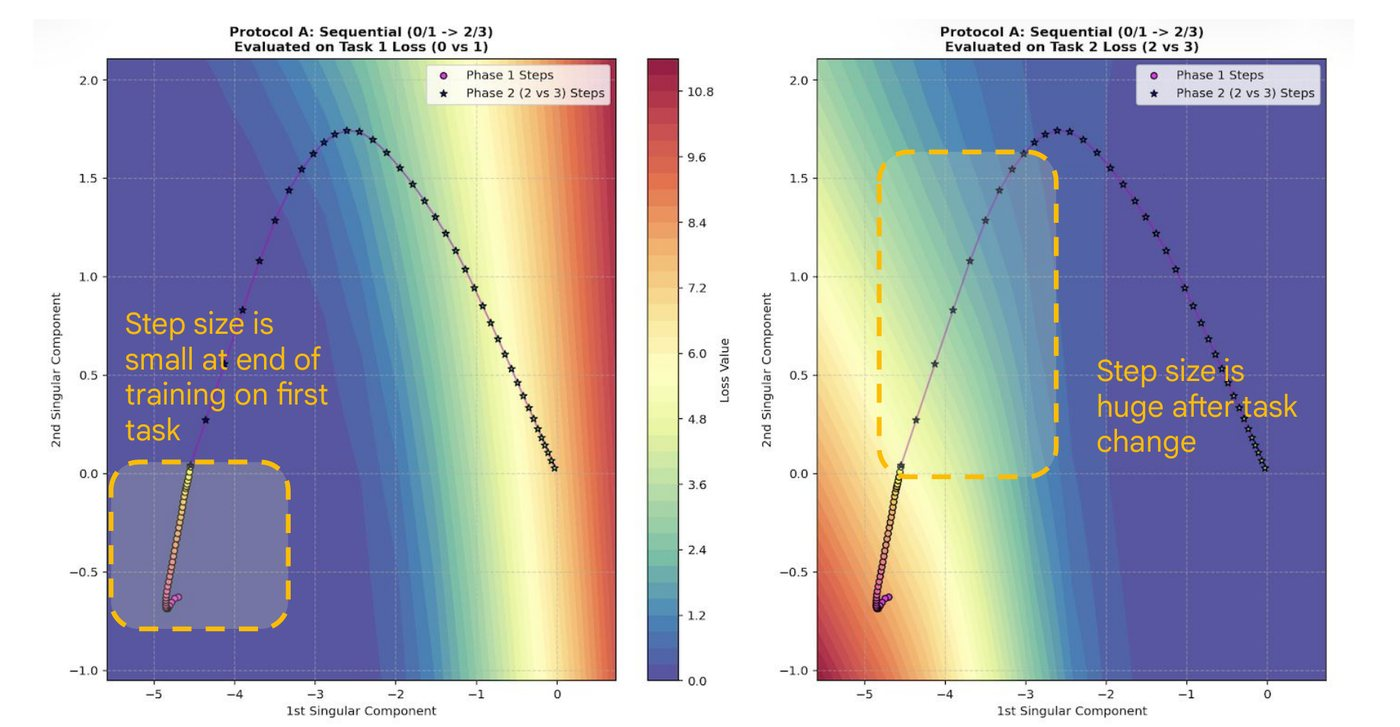
\includegraphics[width=0.90\textwidth]{figures/continual-learning-1.jpg}
\caption{Why plasticity is lost immediately rather than gradually, from the Continual Learning
lecture. The same optimisation trajectory is drawn over the task-one loss surface (left) and
the task-two loss surface (right), projected onto two singular components. Steps are tightly
packed at the end of task one, boxed on the left, and become very large as soon as the loss
switches to task two, boxed on the right. Adam's slow-decaying second moment still reflects
the small gradients of the previous task, so the effective step size overshoots.}
\label{fig:continual-learning-1}
\end{figure}

\paragraph{Why a large step is specifically destructive.} A large step does not merely
overshoot a minimum. It overshoots the receptive field of the nonlinearity: the preactivations
for a unit are pushed outside the range where the activation function is responsive, given the
feature covariance the network had built up. That is how ReLUs die. It also explains why the
remedy is not simply a smaller learning rate but control of the geometry, and it connects to a
neat observation in the lecture on parameter norm: rotating a large parameter vector by a given
angle requires a much larger perturbation than rotating a small one, so unchecked norm growth
makes the network progressively harder to move in function space
(Figure~\ref{fig:continual-learning-3}).

\begin{figure}[htbp]
\centering
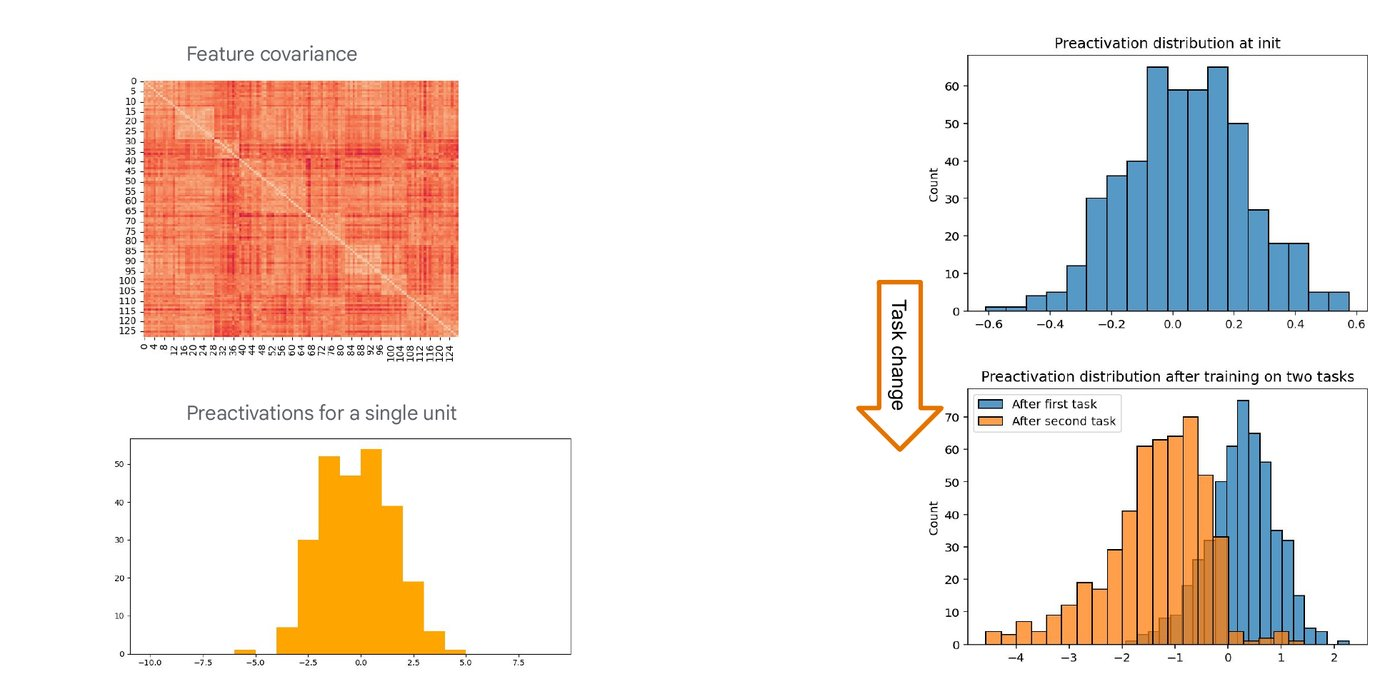
\includegraphics[width=0.90\textwidth]{figures/continual-learning-3.jpg}
\caption{How a large step kills a unit, from the Continual Learning lecture. Left, the feature
covariance the network has built up and the preactivation histogram for one unit. Right, the
same unit's preactivation distribution at initialisation, centred on zero and narrow, and after
training on two tasks: the second task's distribution, in orange, has shifted almost entirely
below zero. Once preactivations leave the range where the activation responds, the unit stops
passing gradient, which is what ``the ReLUs are dead'' means in practice.}
\label{fig:continual-learning-3}
\end{figure}

\paragraph{The fixes are boring.} What Lyle calls the swiss cheese approach
is three complementary interventions: control parameter norm growth, normalise preactivations,
and avoid regressing on ill-conditioned targets. The lesson is stated as use normalisation
layers and do not let parameters get too big. With these in place continual training stabilises
to the degree that the network can memorise effectively unlimited random labels of MNIST, and
the same treatment stabilises reinforcement learning. A separate and non-catastrophic route to
plasticity loss is warm-starting~\citep{ash2020}, tied to primacy bias: early in training a
model makes large changes relative to its current features, later only small ones. The proposed
remedy is to re-warm the effective learning rate above the threshold at which the model still
makes nontrivial changes to its features.

\section*{Notation}

The chapter follows the lecture's informal usage: $\task$ for a task, plasticity discussed
through the effective step size rather than a single symbol. Where the lecture refers to the
empirical NTK matrix it means the Gram matrix of per-example gradients at convergence, used as
a diagnostic of conditioning rather than as a theoretical object.

\section*{Why it matters}

This is the chapter that answers the closing slide of
Chapter~\ref{ch:01-intro-deep-learning}, where Chandar named non-i.i.d.\ learning as the
frontier without saying what breaks. The answer here is specific: the optimiser's state is
stale and the nonlinearity's receptive field is finite. It also stands in productive contrast
with Pascanu (Chapter~\ref{ch:07-to-be-figured-out}), who reaches for the same problem from
the direction of credit assignment and argues something stronger, that the i.i.d.\ assumption
is what makes gradient-based learning work at all. Lyle is the more optimistic of the two: her
position is that most plasticity loss is avoidable with best practices, and that resetting and
distilling remains available as a fallback.

\begin{aside}
The personal notes single out ``catastrophic forgetting'' as the takeaway and ask how to train
networks online. Lyle's answer, read carefully, is partly deflationary: where the data can be
stored, storing it is the right move, and the interesting problem only begins under a memory
constraint. Which regime a project is in decides whether the literature
applies at all, since it is largely written for the constrained case and most applications are
not.
\end{aside}

\chapter[To Be Figured Out]{To Be Figured Out: Inductive Bias, Non-Stationarity
  and Linear Recurrence}
\label{ch:07-to-be-figured-out}
\chaptermark{To Be Figured Out}

\lecturemeta{Razvan Pascanu}{Mila and Google DeepMind}

The title above is the deck's own, and it is accurate: this is a survey of open problems rather
than a result. Its spine is an argument about inductive bias: there is no prior-free machine learning system, every choice
in building one is a bias, and the useful question is therefore not whether to have biases but
which ones buy the most. Pascanu develops that in three registers. Conceptually, the i.i.d.\
assumption is itself a bias doing hidden work, because gradient descent resolves credit assignment
by a tug-of-war between examples and that only works when the data is shuffled. Structurally,
depth and architecture are biases with quantifiable payoffs. Practically, state space models and the
linear recurrent unit buy capability from structure instead of scale, and by the end most of that advantage has evaporated into a hybrid.

\section*{Key ideas}

\paragraph{Why look beyond i.i.d.\ at all.} Four reasons, none of them about benchmark scores.
Scaling is unsustainable, argued with data-centre water and electricity figures rather than
FLOPs. The world is bigger than the agent: models have finite capacity, the world is large and
includes the people modelling it, so continual learning is in a sense unavoidable. Learning on
the fly reframes the goal from asymptotic performance to a tracking question, how well can we
follow a moving target, which makes trade-offs such as compute against performance and
robustness against performance explicit. And efficiency of learning, via
Griffiths~\citep{griffiths2020}: the profile of human intelligence is a consequence of human
limitations, and AlphaGo's move 37 was available precisely because the machine does not
decompose problems into tractable subproblems the way people do, sacrificing performance for
efficiency. Pascanu's hypothesis is that trade-offs are necessary and that limitations should
be exploited to shape the loss surface.

\paragraph{The i.i.d.\ assumption is doing hidden work.} Gradient-based credit assignment inside a
function approximator proceeds by
tug-of-war dynamics between competing examples, which requires the data to be i.i.d. Two consequences are offered as hypotheses, not facts: there is no explicit knowledge
composition, and scale becomes a crutch that makes learning possible at all. Failure of credit
assignment is then what catastrophic forgetting \emph{is}, rather than a separate phenomenon.
The natural inference, that curricula should therefore help, does not survive
contact~\citep{schaul2019, toneva2019}, and the lecture explains why exploiting this is not
easy: we do not know how to measure what we care about when building a representation, and
learning lacks compositionality and locality.

\paragraph{No prior-free learning, and depth as a quantifiable prior.} Priors, regularisers
and inductive biases all restrict or reshape the search space, and since every step in
constructing a system is such a choice, the King Midas framing is that the choice cannot be
declined. Depth is the cleanest example of a bias with a countable payoff: Zaslavsky's
theorem on hyperplane arrangements~\citep{zaslavsky1975} bounds how a single layer partitions
input space, and composing layers multiplies regions, which is the counting argument behind
the number of linear regions of a deep network~\citep{montufar2014}. On optimisation the
lecture is deflationary about the folklore. High-dimensional non-convex loss surfaces are
dominated by saddles rather than bad minima~\citep{dauphin2014}, so the deep learning myth,
that networks can be dropped in anywhere and optimisation behaves as if convex, holds only if
the right protocol is used. Initialisation and the choice of optimiser qualitatively alter which
solution is reached, which Pascanu argues should be leveraged instead of treated as
nuisance; and a loss surface of sufficient dimension contains every low-dimensional
pattern~\citep{czarnecki2019}, which is a warning about reading too much into loss-landscape
visualisations.

\begin{figure}[htbp]
\centering
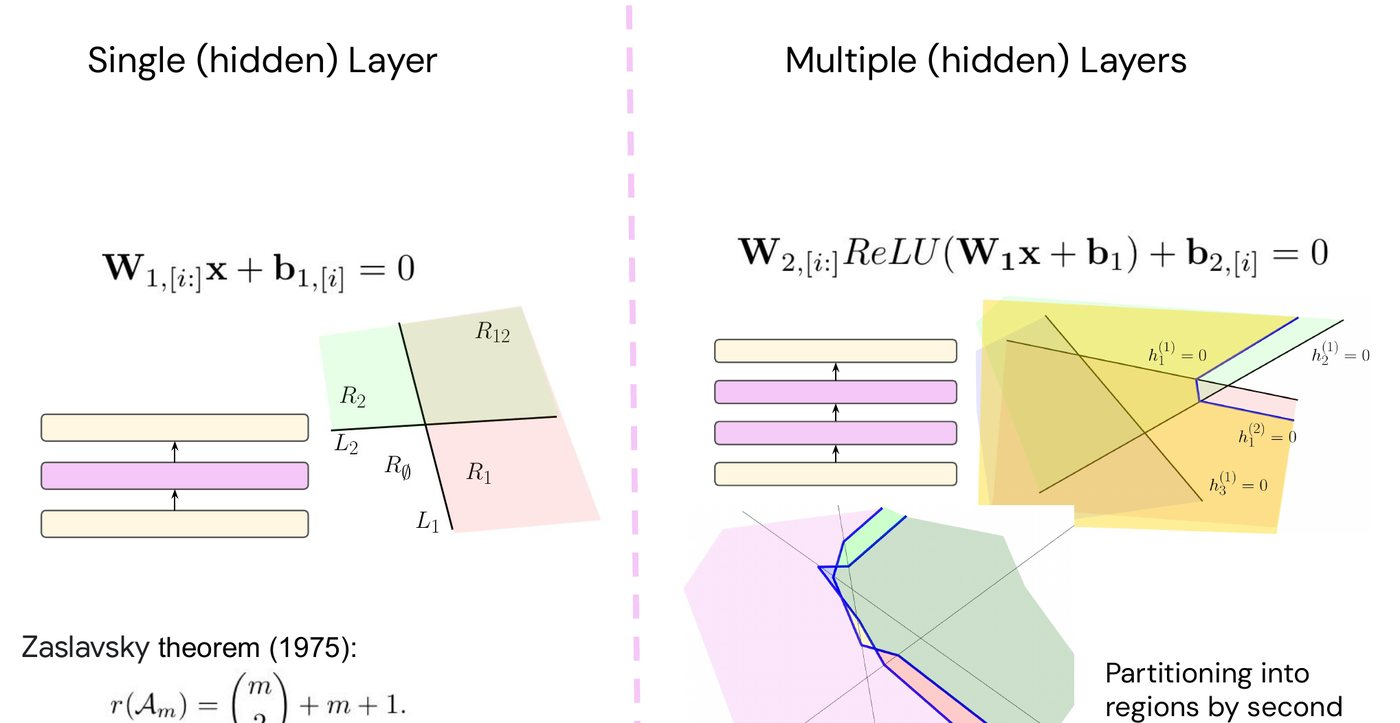
\includegraphics[width=0.80\textwidth]{figures/to-be-figured-out-2.jpg}
\caption{Depth as a bias with a countable payoff, from the To Be Figured Out lecture. A single hidden
layer cuts input space with hyperplanes $\mat{W}_{1,[i:]}\xin + \vect{b}_{1,[i]} = 0$, and
Zaslavsky's formula gives the number of resulting regions. A second layer's boundaries
$\mat{W}_{2,[i:]}\,\mathrm{ReLU}(\mat{W}_1\xin + \vect{b}_1) + \vect{b}_{2,[i]} = 0$ are
piecewise linear, bending as they cross the first layer's regions, so the count multiplies
rather than adds. This is the origami picture of why depth buys expressivity.}
\label{fig:to-be-figured-out-2}
\end{figure}

\paragraph{State space models, and why they are hard to reason about.} The second half opens
with a hardware question: are transformers optimal? The worry is inference cost, usually framed
as the quadratic cost of attention, and the comparison the lecture draws is per-step: recurrence
is $O(1)$, attention $O(N)$. State space models are the community's main answer, and Pascanu
describes them as a variant of linear RNNs. An SSM models the sequence in continuous time,
relies on a deterministic HiPPO initialisation, and is then discretised; the payoff is that the
discretised system can be read either as a recurrence, which makes inference fast, or as a
convolution, which makes training fast. That dual view is the whole appeal.

His objection is methodological, not empirical. There are many variants (S4~\citep{gu2022s4},
S4D, H3, Mamba~\citep{gu2023mamba}), several discretisation schemes such as bilinear and
zero-order hold, it is unclear how changes to the surrounding block interact with the SSM's
parameterisation, and for the better-performing SSMs the continuous-time story becomes
strenuous. The question he poses is how to disentangle which ingredient is actually doing the
work.

\paragraph{The LRU as an ablation, not a new model.} The linear recurrent unit is the answer to
that question, derived in six steps~\citep{orvieto2023}. Start from a transformer backbone,
because the MLP supplies the expressivity and therefore the recurrent block is allowed to be
simple. Remove the nonlinearity from the recurrence, which costs less than expected: linear
RNNs followed by nonlinear projections can approximate any finite sequence-to-sequence map, with
the linear recurrence compressing the sequence and the MLP approximating the decompressor. The
caveat is stated, that this construction can only exhibit fading memory. Linearity then permits
diagonalisation, so a complex diagonal $\Lam$ is learned directly and the recurrent computation
collapses, and stability becomes a statement about eigenvalues: inside the unit disk gives
exponentially decaying sine waves, outside is unstable. Vanishing gradients are the mirror
image, since eigenvalues near the origin decay within a few steps, so initialisation samples an
annulus that excludes the origin, typically $r_{\min} = 0.9$ and $r_{\max} = 0.999$
(Figure~\ref{fig:to-be-figured-out-1}). Stable parameterisation and normalisation, the latter
needed to control hidden-state growth, complete the recipe.

The results that matter here are the negative ones. HiPPO is not necessary. Continuous time is
not necessary. Complex numbers may be doing nothing more than providing a compact
representation, since a symmetric real system can perform similar computations at the cost of a
larger state. In other words, most of the conceptual apparatus that SSM papers carry is
detachable, and what remains is a diagonal linear recurrence with a sane spectrum. The lecture
then descends to hardware, noting a roughly eightfold gap between HBM and VMEM transfer rates on
the TPU profiled, and that a linear RNN performs an associative scan and so parallelises across
time despite being a recurrence.

\begin{figure}[htbp]
\centering
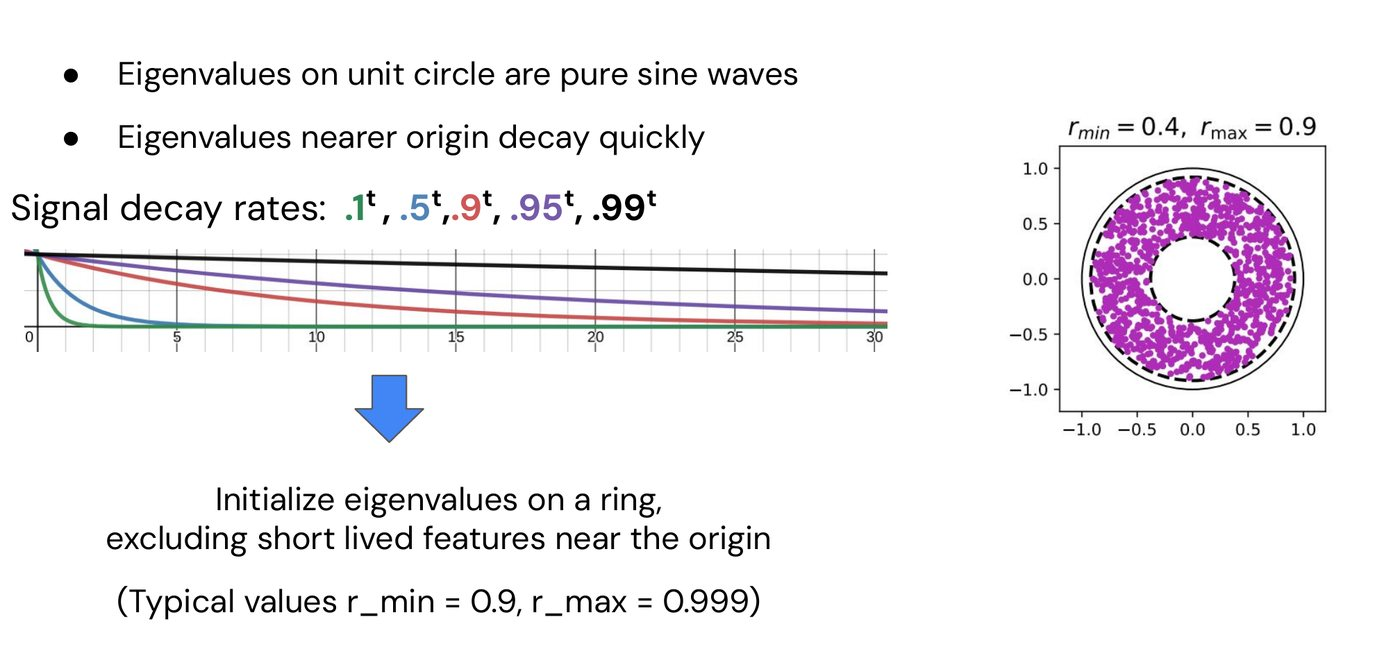
\includegraphics[width=0.82\textwidth]{figures/to-be-figured-out-1.jpg}
\caption{Step three of the linear recurrent unit derivation, from the To Be Figured Out
lecture. Left, signal decay $r^{t}$ for $r$ from $0.1$ to $0.99$: an eigenvalue of modulus
$0.5$ has effectively forgotten its input within five steps, while $0.99$ persists past thirty.
Right, the consequence for initialisation, eigenvalues sampled from an annulus rather than a
disk so that no unit starts with a memory too short to be useful. The annulus drawn uses
$r_{\min} = 0.4$, $r_{\max} = 0.9$; the values recommended in practice are $0.9$ and $0.999$.}
\label{fig:to-be-figured-out-1}
\end{figure}

\paragraph{The scorecard, and the hybrid that actually wins.} Having built the case,
Pascanu reports that pure recurrence does not straightforwardly win. On language S4D did not work
out of the box and an LSTM was better; gating it helped. What does work is a hybrid, and the
reasoning is that SSMs and linear attention share the two properties that matter, a finite state
and linear scaling in sequence length, while being complementary in what they capture: the SSM
models the whole sequence, linear attention captures local information. The recipe given is a
block pattern repeating two SSM blocks to one linear-attention block, and the configuration
reported as state of the art at scale is roughly 75\% linear attention with 25\% global softmax
attention retained (Figure~\ref{fig:to-be-figured-out-3}). As models scale, behaviour and
limitations converge, so the remaining gains are situational: online inference, and scaling down
by distillation. The closing summary keeps
both halves: biases are unavoidable, continual learning may be the next change of perspective,
scale might work but is not the only option, transformers rely on a factorisation of simple
components that must be scaled, and attention might not be all we need.

\begin{figure}[htbp]
\centering
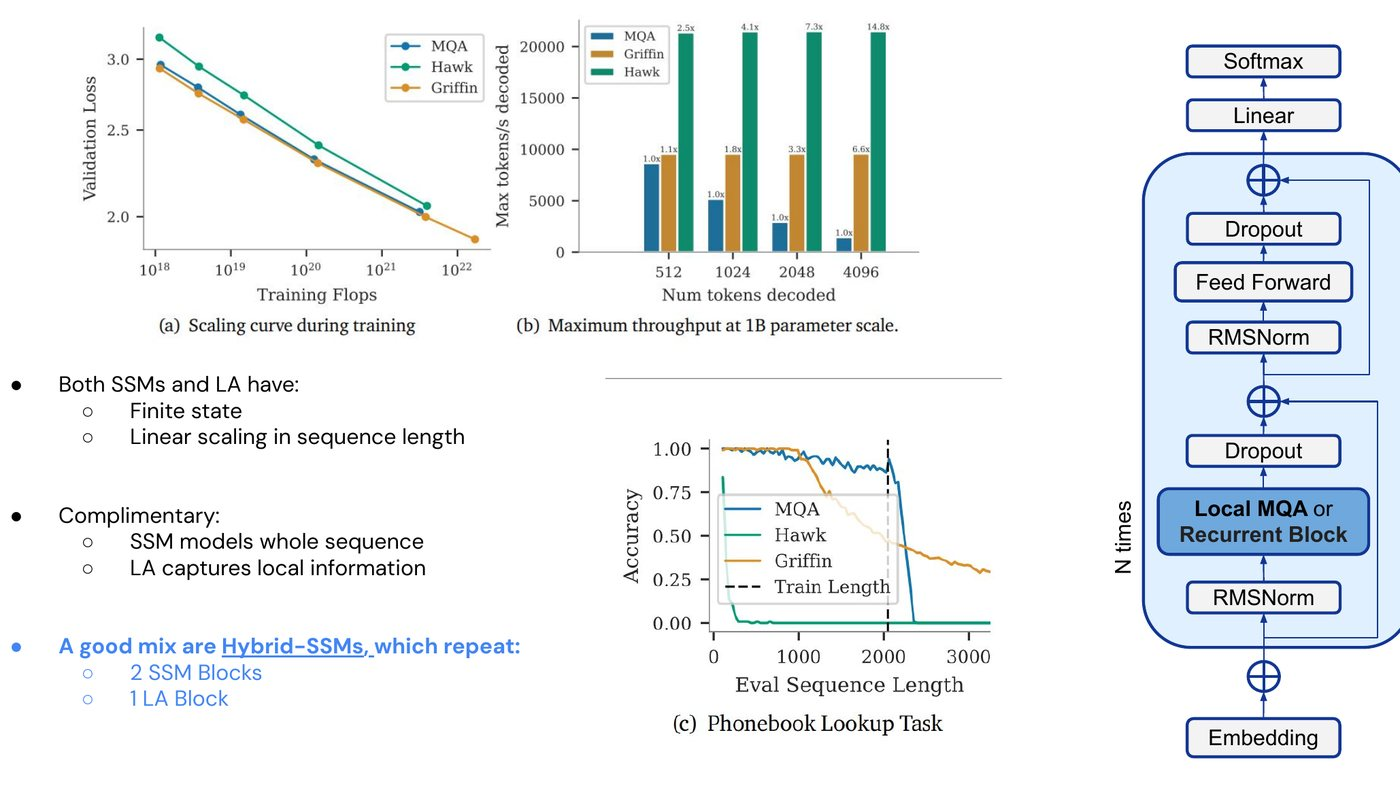
\includegraphics[width=0.86\textwidth]{figures/to-be-figured-out-3.jpg}
\caption{What actually wins, from the To Be Figured Out lecture. Left, the case for hybrids:
state space models and linear attention share a finite state and linear scaling in sequence
length, and are complementary because the SSM models the whole sequence while linear attention
captures local structure. Middle, the evidence, with matched scaling curves, an order-of-magnitude
throughput advantage at 1B parameters, and a phonebook-lookup task where the pure recurrent
variants degrade past their training length. Right, the resulting block, alternating a recurrent
or local-attention block with feed-forward layers.}
\label{fig:to-be-figured-out-3}
\end{figure}

\section*{Notation}

$\Lam$ denotes the diagonal matrix of recurrence eigenvalues, $r$ their modulus, $t$ discrete
time. The lecture uses $\theta$ for parameters as elsewhere in this book, and writes
$\theta_0$, $\theta_{\text{generalize}}$ and $\theta_{\text{overfit}}$ for points in parameter
space when discussing capacity, which is retained here in prose rather than symbols.

\section*{Why it matters}

Read this immediately after Chapter~\ref{ch:06-continual-learning}, because Lyle and Pascanu
disagree in an interesting way. Lyle treats plasticity loss as a set of fixable engineering
faults in the optimiser and the architecture; Pascanu treats the same territory as evidence
that gradient-based credit assignment is structurally dependent on i.i.d.\ data, which is a
much stronger claim and would mean the fixes are palliative. The linear-recurrence material
also connects to Chapter~\ref{ch:10-efficient-learning}: both lectures end up at the same
place, that the binding constraint is memory bandwidth rather than arithmetic, and both reach it
from opposite directions. The personal note to ``check the MAMBA paper'' belongs
here~\citep{gu2023mamba}, with the caution that Pascanu's point is precisely that Mamba's
continuous-time framing is not what makes it work.

\begin{aside}
Pascanu's deck borrows three slides from Kyunghyun Cho on language modelling, and cites the
statistics view that firing a linguist improves the recogniser. Set against
Chapter~\ref{ch:05-statistics-estimation}, where Cho argues for learning the estimator rather
than modelling the process, the two speakers are making the same argument from different ends:
Cho says the generative process need not be modelled, Pascanu says some prior about it is
unavoidable. Both are right, and what is left over is the question of which biases are cheap to
state and expensive to learn.
\end{aside}

\chapter{ML for Mathematics}
\label{ch:08-ml-for-mathematics}

\lecturemeta{Matija Tapu\v{s}kovi\'{c}}{University of Oxford}

Tapu\v{s}kovi\'{c} is a mathematician rather than a machine learning researcher, and the talk
asks one question: can machine learning discover new mathematics? The answer is organised into
three strands, learning from examples, searching in language space, and formalisation, and the
recurring test applied to each is the one a mathematician would apply: where does the machine's
output re-enter mathematics? Not whether a metric improved, but whether the result becomes a
theorem, a conjecture someone will chase, or merely a number. The conclusion running through all
three strands is that the search is rarely the bottleneck. Building a cheap, exact and
ungameable evaluator is the research.

\section*{Key ideas}

\paragraph{Strand I, learning from examples, works when attribution is interpretable.} The
flagship result is on Kazhdan--Lusztig polynomials. A permutation becomes a directed graph, an
interval $[x,y]$ in the Bruhat order becomes a subgraph, and the combinatorial invariance
conjecture of Lusztig and Dyer says isomorphic unlabelled interval graphs give the same
polynomial. A message-passing GNN was trained on the bare interval graph to predict the
coefficients of $P_{x,y}$, and gradient attribution flagged particular edges as
overrepresented~\citep{davies2021}. Those flagged edges pointed at a decomposition: a recipe
computes $P_{x,y}$ from a split of the interval into two smaller pieces, though the recipe needs
labels, and the new conjecture is that any valid split agrees, which would imply combinatorial
invariance (Figure~\ref{fig:ml-for-mathematics-1}). A variant of that conjecture has since been
proved for broad families. The point is that the network's value was not its accuracy but the
fact that its attribution was legible enough to become a mathematical statement.

\begin{figure}[htbp]
\centering
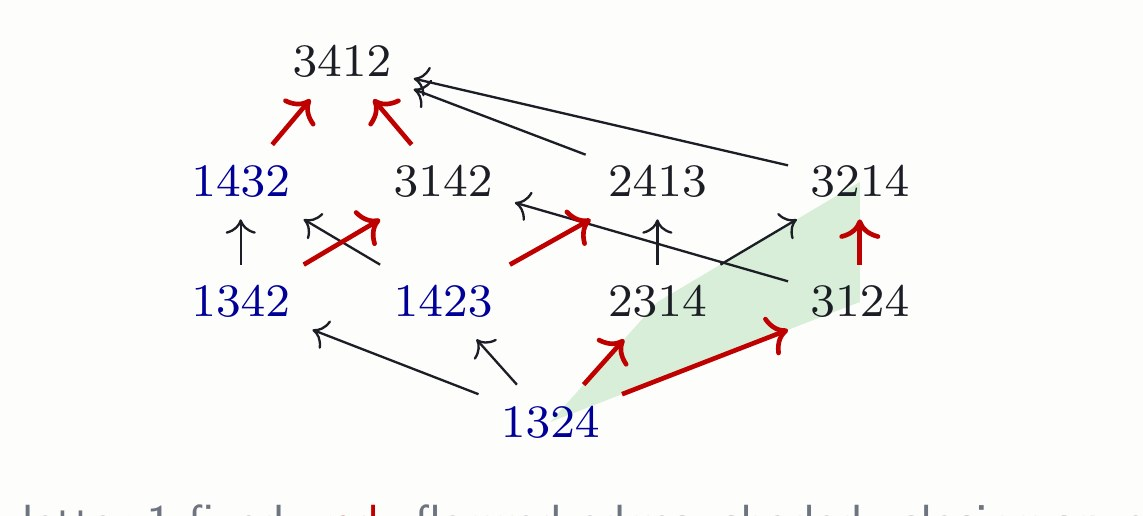
\includegraphics[width=0.68\textwidth]{figures/ml-for-mathematics-1.jpg}
\caption{The output that re-entered mathematics, from the ML for Mathematics lecture. An
interval in the Bruhat order on permutations, drawn as a directed graph. Red marks the edges
that gradient attribution on the trained GNN flagged as overrepresented, blue marks vertices
whose first letter is fixed, and the shaded region is the closing square of the split those
flagged edges suggested. This picture, not the model's accuracy, is what became a conjecture.}
\label{fig:ml-for-mathematics-1}
\end{figure}

\paragraph{The counterexample in the same strand is instructive.} On elliptic curves
$E: y^2 = x^3 + Ax + B$, the rank in
$E(\mathbb{Q}) \cong E(\mathbb{Q})_{\text{tors}} \oplus \Z^{\rank(E)}$ is not directly
computable, so the experiment represented each curve by its sequence of point counts
$a_p = (p+1) - N_p(E)$ and ran logistic regression on $(a_2, a_3, \dots) \in \Z^{500}$ to
separate rank 0 from rank 1, reaching over 97\% accuracy and beating known
heuristics~\citep{he2022}. The expert reaction quoted on the slide is the lesson: what has been
learned is the sign in the functional equation of the associated $L$-function, not the rank. The
model was right for a reason that made it uninformative, and the data came from an archive
rather than a generator, which limits what could be probed.

\paragraph{A worked case study in why data, not method, is the constraint.} The Feynman-integral
material is the most detailed part of the lecture and reads as a cautionary tale told against
the speaker's own field. The question is whether weight drop, conjecturally equivalent to
$c_2 = 0$, is visible in elementary graph features. On 1,958 graphs up to 11 loops with 272
positives and 24 features, AUC was 0.90. Then the deflation begins. The top feature restates a
known theorem, that a 3-vertex cut forces a product and hence $c_2 = 0$; remove those positives
and AUC falls to 0.85. The 165 survivors form only 7 families with labels constant within a
family, so the classifier is largely recognising disguised siblings; hold out whole families and
AUC falls to 0.74. In the full catalogue of 283 irreducible families up to 10 loops, exactly 7
have the drop, and those 7 are conspicuous anyway, with automorphism groups roughly twenty times
larger than typical and degenerate, often integer, spectra. With 7 positives the finding is a
description, not a rule. Two further constraints are named: labels are genuinely expensive, since
at 11 loops $c_2$ is known at only four primes and the next prime can cost hours per graph; and
GNNs are the wrong tool here because $\phi^4$ graphs are 4-regular, so a message-passing network
is blind by 1-WL to exactly the signal that works, which points at the geometric deep learning
toolkit as the fix (Chapter~\ref{ch:11-geometric-deep-learning}).

\paragraph{Strand II, search in language space, when there is no dataset.} The reframing is that
a scoring function is enough to enable search, and the key move is not to search the space of
objects but the
space of programs that generate them, so that a program inherits the score of its output and an
LLM proposes variants. The lineage given runs from extremal-combinatorics search through
PatternBoost to FunSearch and AlphaEvolve. The flagship evaluation is 67 problems, hours each,
almost all of the form improve a bound on a constant, with a scorecard of 20 new, 39 matched and
8 fell short~\citep{georgiev2025}. The authors' own framing is quoted rather than softened: none
of the results is individually important, every one could have been found with standard tools, and
the point is time; the tool beats the literature where the literature is thin and matches or
trails it where it is deep. The concrete highlight is Kakeya and Nikodym sets over finite fields,
where the previous Kakeya record in dimension three was
$\tfrac14 p^3 + \tfrac78 p^2 + O(p)$ and AlphaEvolve found
$\tfrac14 p^3 + \tfrac78 p^2 - \tfrac18$ for $q = p \equiv 1 \bmod 4$, a two-line formula over
quadratic residues. For Nikodym sets the machine's idea, delete surfaces rather than points, was
no better than random as used, and a human repaired it by hand into a genuine improvement. The
recurring observation is that the expertise moved into the evaluator.

\paragraph{Strand III, certainty.} A proof assistant checks that a term inhabits a type, so
compiling a statement establishes well-formedness, not truth, and the proof term is what must be
constructed. The motivating question is sharp: would any expert read a 150-page proof of a major
conjecture handed over by a language model? Formal infrastructure is
uneven, with mathlib at roughly 2.3M lines built over nine years, covering approximately an
undergraduate degree and jagged beyond it. The competition trajectory given is 2024 AlphaProof
and AlphaGeometry at silver with the kernel as evaluator, 2025 Deep Think at gold in plain
English graded by humans, and 2026 AxiomProver at 42 out of 42, formal end to end, roughly 8,000
lines of Lean in about 25 hours. The research-level example
closes the loop: for minimal Kakeya sets in $\mathbb{F}_p^3$, AlphaEvolve found the construction,
Deep Think proved it and AlphaProof certified it, the full pipeline closed, but only because every
ingredient was already in mathlib. In dimension 4 elliptic curves appear and the certification
fails; for Nikodym sets the construction was too tangled to analyse and the final proof was
entirely human. The frontier of machine certification runs out precisely where the deep objects
begin.

\section*{Notation}

$S_n$ is the symmetric group, $P_{x,y}(q)$ a Kazhdan--Lusztig polynomial, $E$ an elliptic curve
with $a_p$ its trace of Frobenius at $p$, $c_2$ the Feynman-graph invariant whose vanishing is
weight drop, and $\pi(x)$ the prime counting function.

\section*{Why it matters}

This chapter is a rigorous account of what it takes for a machine learning result to count as a
contribution in a field with an external standard of correctness, which makes it the sharpest
methodological lecture of the week. Its central complaint, that the evaluator is the research and
the search is not the bottleneck, transfers directly to reinforcement learning
(Chapter~\ref{ch:04-intro-reinforcement-learning}), where RLVR is exactly the claim that a
cheap, exact, ungameable reward changes what is learnable. The Feynman-graph observation that
4-regularity makes message passing blind is a concrete instance of the expressivity limits that
Chapter~\ref{ch:11-geometric-deep-learning} addresses by construction.

\begin{aside}
The three strands are an escalating standard of evidence, and the same ladder can be applied to
ordinary machine learning work. Strand I asks whether a model's attribution
is legible enough to state as a claim. Strand II asks whether the score is faithful enough that
optimising it means something. Strand III asks whether the result can be checked without trusting
the producer. Most machine learning papers only clear the second bar, and clear it against a
metric far less exact than a Lean kernel.
\end{aside}

\chapter{Spectral Analysis of Directed Acyclic Graphs}
\label{ch:09-spectral-analysis-dags}

\lecturemeta{Isidora Stankovi\'{c}}{Faculty of Electrical Engineering, University of Montenegro}

One obstruction, one construction, one proof that the construction costs nothing. Graph signal processing supplies a Fourier transform by
diagonalising the adjacency matrix, and on a directed acyclic graph that machinery fails
completely, because a DAG's adjacency matrix is nilpotent and therefore has every eigenvalue
equal to zero. Stankovi\'{c}'s answer is to add a return edge to close the graph into a cycle,
which restores a spectrum, and then to insert enough zero-valued vertices along that return path
that the feedback it introduces cannot reach the original vertices within the filter's horizon.
The spectrum comes back and the filter output on the original graph is unchanged.

\section*{Key ideas}

\paragraph{Why anyone should care about DAG spectra.} DAGs are everywhere in machine learning:
computation graphs, causal and Bayesian networks, and autoregressive models, where causal
attention is precisely a DAG. The graph Fourier transform is the basis for spectral GNNs and for
graph filtering, so if it degenerates on DAGs then an entire toolkit is unavailable on a class of
graphs we use constantly.

\paragraph{The setup, in one paragraph.} For a directed graph $G = (V,E)$ with $|V| = N$ and
adjacency matrix $\Adj$, a graph signal is $\gsig = [x(1), \dots, x(N)]\T$. The shift operator is
the adjacency matrix itself, and a linear graph system is a polynomial in it,
\[
  H = \sum_{s=0}^{S} h_s \Adj^{s}, \qquad y = H\gsig = \sum_{s=0}^{S} h_s \Adj^{s}\gsig,
\]
\noindent where $\Adj^{s}$ describes propagation along directed paths of length $s$. This is
graph convolution: $\Adj\gsig$ is one message-passing hop and the $h_s$ are exactly the
coefficients a spectral GNN learns. If $\Adj = \Vmat \Lam \Vmat\inv$ is diagonalisable, the GFT is
$X = \Vmat\inv \gsig$ and the system acts multiplicatively in the spectral domain,
$H(\Lam) = \sum_s h_s \Lam^{s}$.

\paragraph{The obstruction is structural, not numerical.} Topologically order a DAG's vertices
and its adjacency matrix becomes strictly upper triangular, which the lecture notes has the same
shape as a causal attention mask. A strictly upper triangular matrix is nilpotent,
$\Adj^{K} = \vect{0}$ for large enough $K$, so every eigenvalue is zero and $\Lam = \vect{0}$.
The consequence is not a loss of precision but a total collapse:
\[
  H(\Lam) = \sum_{s=0}^{S} h_s \Lam^{s} = h_0 \id,
\]
\noindent so every graph mode has the identical gain $h_0$, spectral components become
indistinguishable, frequency ordering disappears, and the adjacency-based GFT loses all
interpretability. What survives is vertex-domain propagation: $\Adj^{s}\gsig$ is still perfectly
meaningful. The spectrum, not the graph, is what breaks.

\begin{figure}[htbp]
\centering
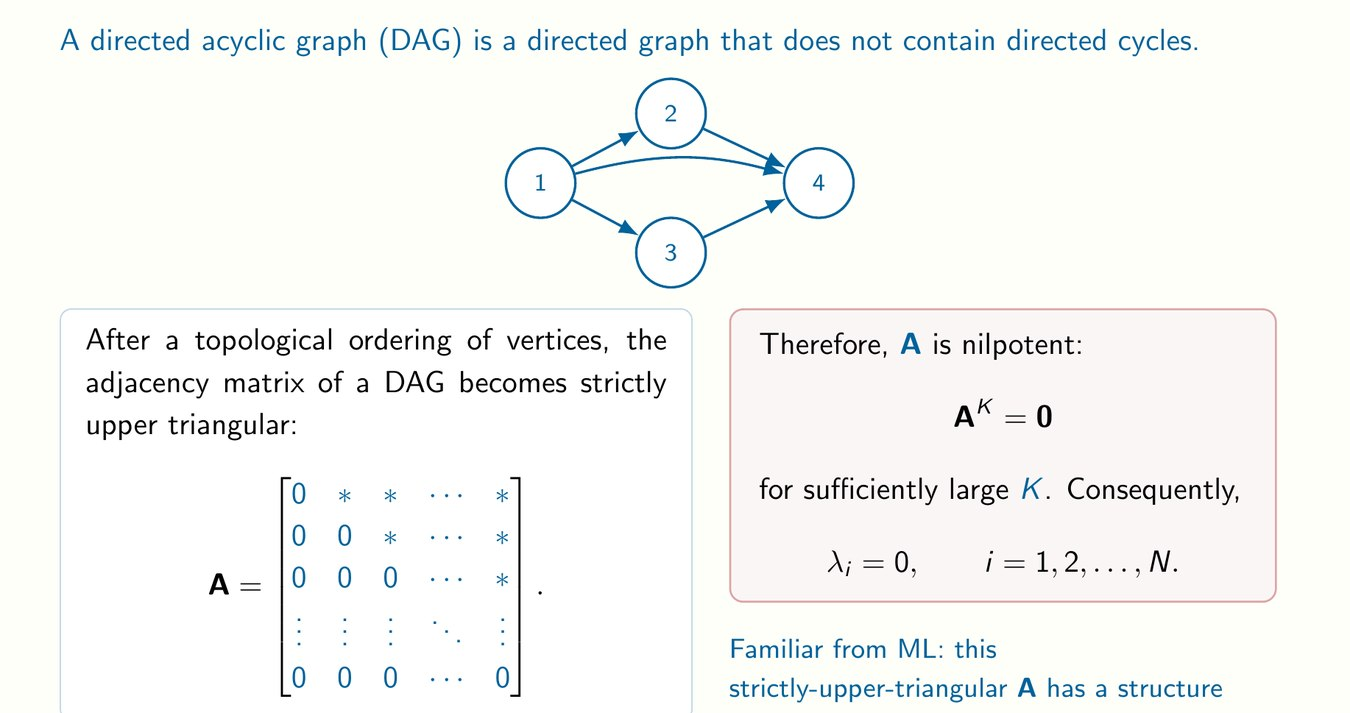
\includegraphics[width=0.86\textwidth]{figures/spectral-analysis-dags-1.jpg}
\caption{Where the obstruction comes from, from the Spectral Analysis of DAGs lecture. Topologically
ordering a DAG's vertices makes the adjacency matrix strictly upper triangular, which forces
$\Adj^{K} = \vect{0}$ and hence $\lambda_i = 0$ for every $i$. The lecture's own aside, bottom right: this is the same
matrix structure as a causal attention mask, so every decoder-only transformer has the same
degenerate spectrum.}
\label{fig:spectral-analysis-dags-1}
\end{figure}

\paragraph{Zero-padding, and the analogy that motivates it.} The construction is borrowed from
classical DFT practice (Figure~\ref{fig:spectral-analysis-dags-2}). A finite signal has no
spectrum until it is extended periodically, which introduces circular wrap-around; zero-padding is
how signal processing prevents that wrap-around from contaminating the interval of interest. The
graph version runs in three steps. A directed path has no spectrum because propagation does not
wrap around. Add a return edge from sink to source and the graph becomes a cycle, whose adjacency
eigenvalues are $\lambda_k = e^{j 2\pi (k-1)/N}$ with complex-exponential eigenvectors, so graph
spectral analysis on the cycle coincides exactly with the classical DFT. But the return edge is
feedback. So insert $M \ge S$ zero-valued vertices along it, which delay that feedback past the
horizon of any filter of order $S$.

\begin{figure}[htbp]
\centering
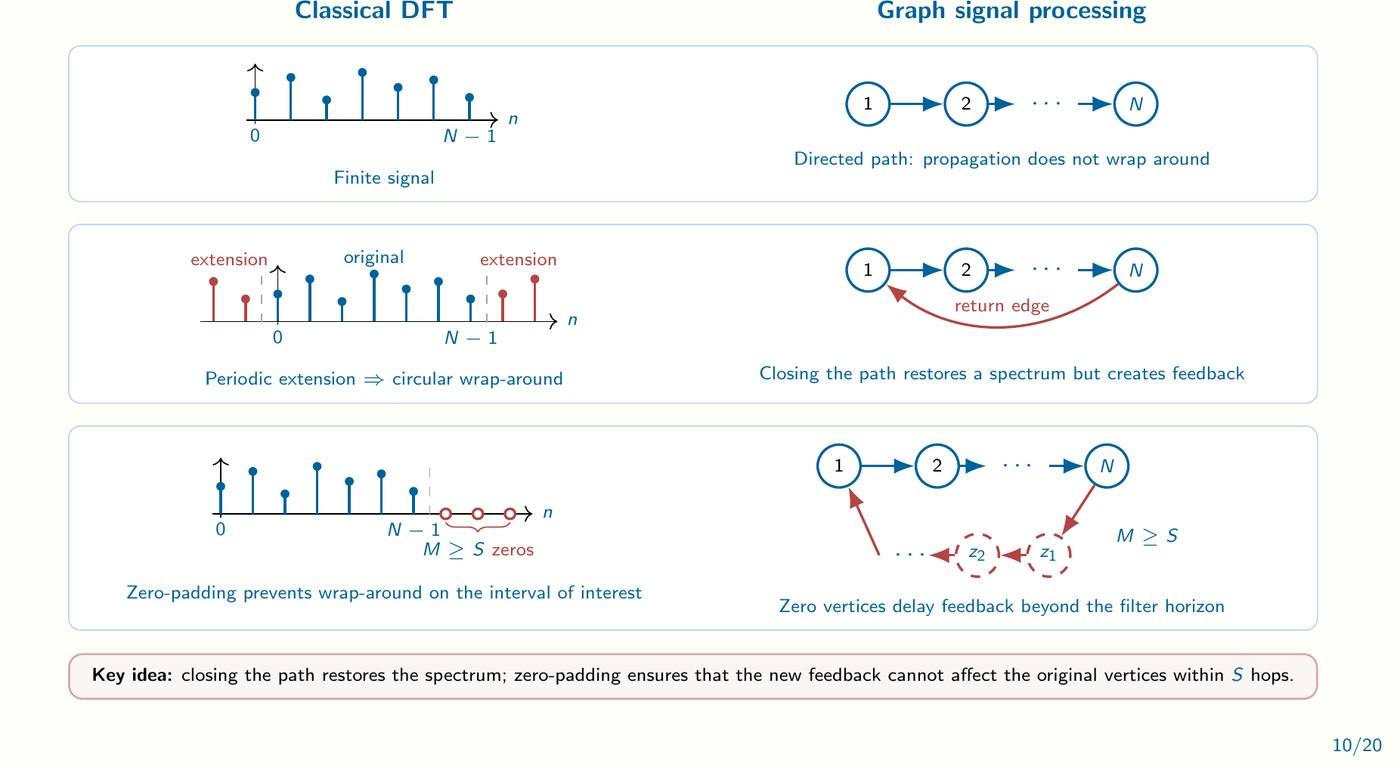
\includegraphics[width=0.92\textwidth]{figures/spectral-analysis-dags-2.jpg}
\caption{The construction and the analogy it comes from, from the Spectral Analysis of DAGs
lecture. Left column, classical DFT: a finite signal has no spectrum, periodic extension supplies
one at the cost of circular wrap-around, and zero-padding pushes that wrap-around outside the
interval of interest. Right column, the graph version step for step: a directed path does not wrap
around, a sink-to-source return edge closes it and restores a spectrum but introduces feedback, and
$M \ge S$ zero vertices $z_1, z_2, \dots$ along the return path delay that feedback beyond the
horizon of any order-$S$ filter.}
\label{fig:spectral-analysis-dags-2}
\end{figure}

\paragraph{The guarantee, and why the cycle is not cheating.} The augmented graph is cyclic on
purpose; the original object is still a DAG and the larger graph is a spectral embedding used only
for the transform. The formal statement is that for $0 \le s \le S$,
\[
  \bigl(\azp^{s} \gsig_{\mathrm{ZP}}\bigr)_{1:N} = \Adj^{s}\gsig,
  \qquad \gsig_{\mathrm{ZP}} = \begin{bmatrix} \gsig \\ \vect{0}\end{bmatrix},
\]
\noindent so filter outputs on the original vertices satisfy
$y_{\mathrm{ZP}}(1{:}N) = y$ exactly. After padding, $\azp$ has determinant $\pm 1$ and so is
invertible, meaning no eigenvalue is zero; the eigenvalue angle $\omega_k = \arg\{\lambda_k\}$
becomes the graph frequency, with slow modes at small angles and fast modes at large ones, and a
Fourier-like interpretation is restored. Diagonalisability additionally needs distinct
eigenvalues, which the talk checks exhaustively rather than assuming: over all connected DAGs on
7 vertices, a bare sink-to-source edge gives 98.4\% diagonalisable and one padding vertex gives
99.97\%; on 8 vertices, 99.0\% and, with two padding vertices, 99.91\%. The residual cases resolve
by giving the added edge weight $0.5$.

\begin{figure}[htbp]
\centering
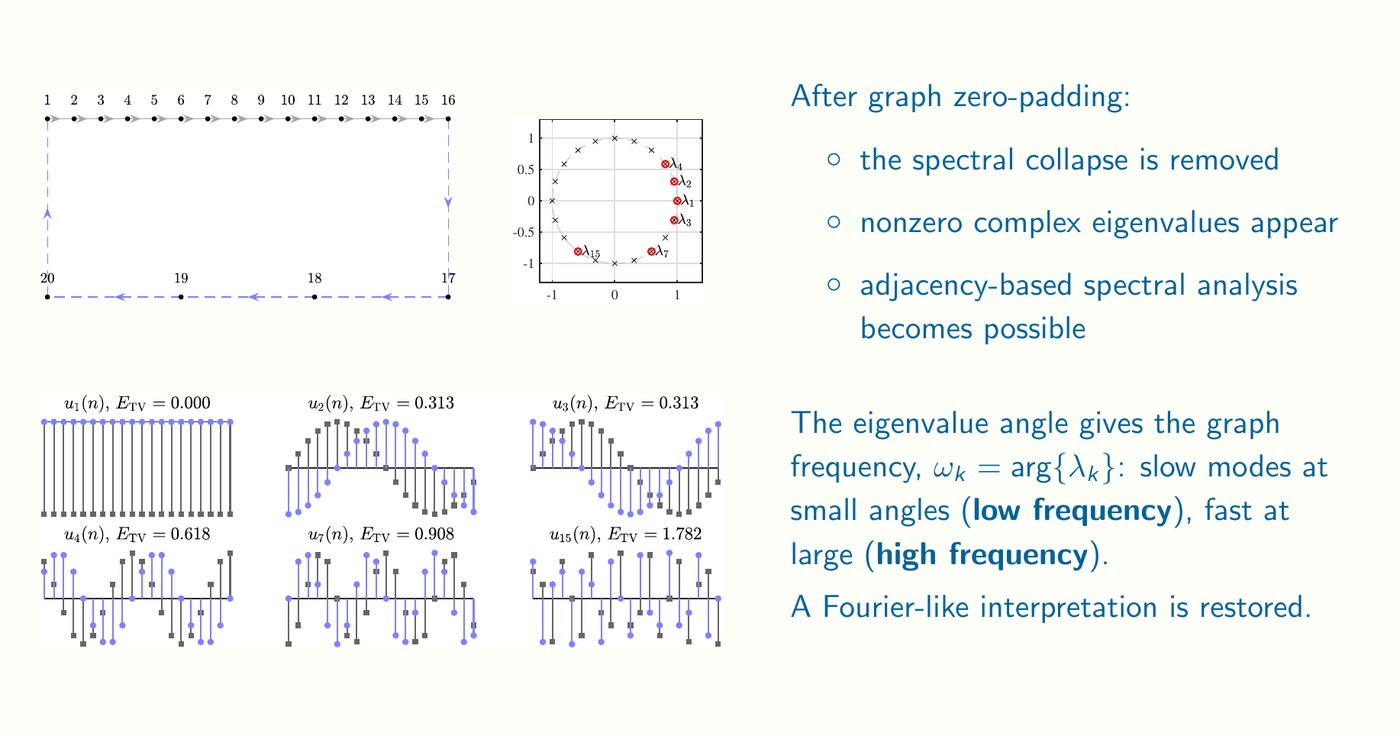
\includegraphics[width=0.92\textwidth]{figures/spectral-analysis-dags-3.jpg}
\caption{What is recovered, from the Spectral Analysis of DAGs lecture. Top left, a zero-padded
graph on 16 original vertices with the padding path closing it. Top middle, the resulting
eigenvalues, now nonzero complex numbers spread around the unit circle rather than all collapsed at
the origin. Bottom left, the corresponding eigenvectors ordered by total variation $E_{\mathrm{TV}}$,
from a constant mode at $0.000$ to a rapidly oscillating one at $1.782$, which is exactly the
low-to-high frequency ordering a Fourier basis is supposed to provide.}
\label{fig:spectral-analysis-dags-3}
\end{figure}

\paragraph{General DAGs, and the cost.} A single return edge suffices only when one directed
Hamiltonian path visits every vertex. A general DAG has several sources and sinks and no such
path, so the pipeline is two-stage: connect the DAG so a Hamiltonian path exists, then pad every
added edge. The overhead is linear, $N_{\mathrm{ZP}} = N + (K+1)M$ vertices for $K$ connecting
edges with $M$ padding vertices each. The worked application is denoising: a graph filter designed
in the restored spectral domain preserves the smoothest spectral components while attenuating
noise-dominated ones, taking a synthetic example from $\snr_{\mathrm{in}} = -6.99$ dB to
$\snr_{\mathrm{out}} = 6.21$ dB (Figure~\ref{fig:spectral-analysis-dags-4}).

\begin{figure}[htbp]
\centering
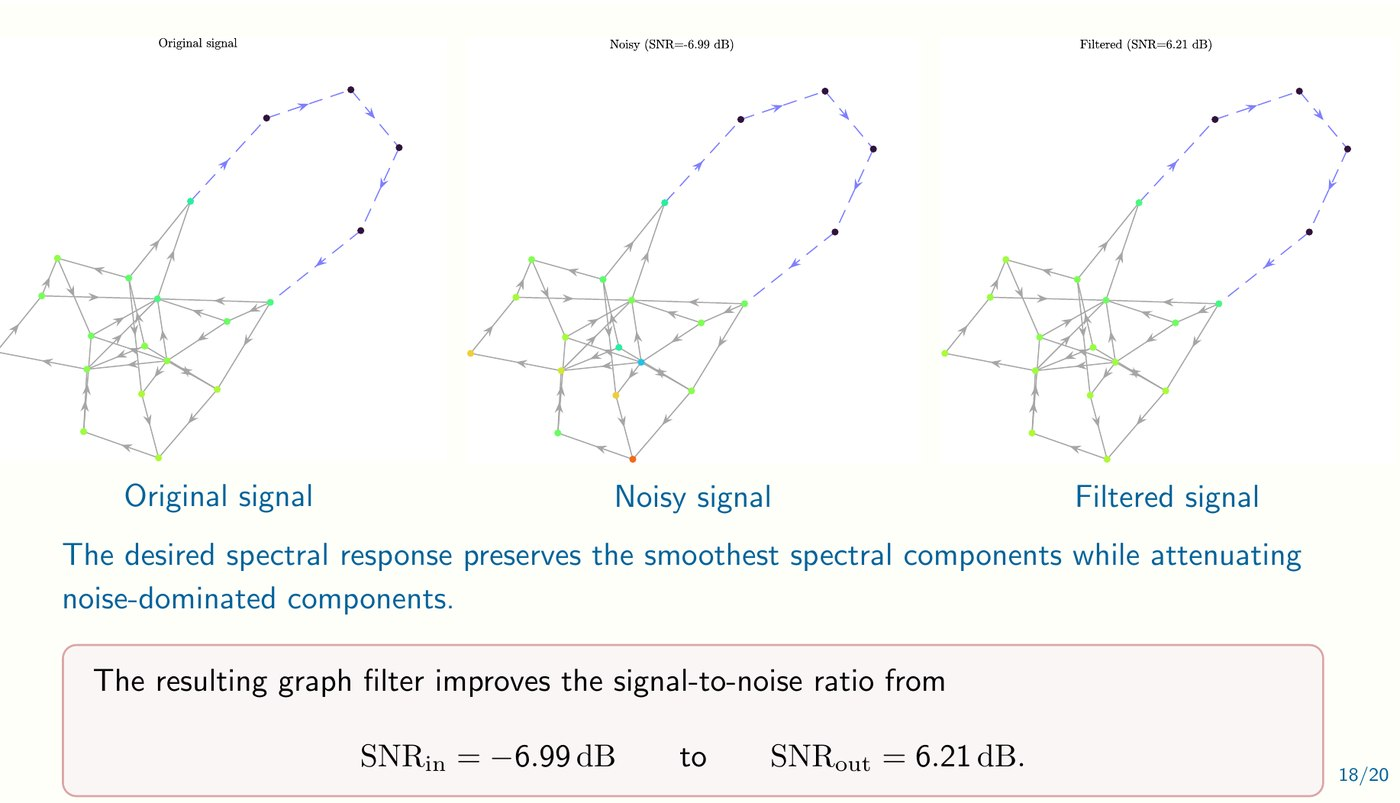
\includegraphics[width=0.92\textwidth]{figures/spectral-analysis-dags-4.jpg}
\caption{The payoff, from the Spectral Analysis of DAGs lecture. The same DAG carrying a smooth
signal, that signal with noise added, and the result of applying a low-pass graph filter designed in
the restored spectral domain. Vertex colour is signal value. The filter is only expressible because
zero-padding gave the DAG a spectrum to design in, and it recovers roughly 13 dB.}
\label{fig:spectral-analysis-dags-4}
\end{figure}

\section*{Notation}

$\Adj$ is the adjacency matrix, $\azp$ its zero-padded counterpart, $\Vmat$ and $\Lam$ the
eigenvector and eigenvalue matrices, $\gsig$ a graph signal, $h_s$ filter coefficients, $S$ the
filter order and $M$ the number of padding vertices. Note the collision with
Chapter~\ref{ch:04-intro-reinforcement-learning}, where $S$ is the state space; here $S$ is a
filter order, following each speaker's own usage.

\section*{Why it matters}

The lecture's own hook, that a strictly upper triangular adjacency matrix looks like a causal
attention mask, is the connection to chase. It means every decoder-only transformer is a DAG
whose spectral analysis is currently unavailable, and this construction is a candidate route to
it. That places the talk directly between Dieleman's spectral view of diffusion
(Chapter~\ref{ch:03-diffusion-models}), which treats the spectrum as the object being generated,
and Veli\v{c}kovi\'{c}'s geometric deep learning (Chapter~\ref{ch:11-geometric-deep-learning}),
where the graph Fourier transform underwrites spectral GNNs. It is also a good model of a small,
complete contribution: an obstruction, a fix, a proof that the fix is free, and an exhaustive
check of the one assumption that could fail.

\begin{aside}
The construction's soft spot is not the spectrum but the requirement of distinct eigenvalues. Instead
of assuming genericity, the talk enumerates all $2^{21}$ connected DAGs on eight vertices and reports
the failure rate. A complete enumeration on small instances costs an afternoon.
\end{aside}

\chapter{Computationally-Efficient Learning}
\label{ch:10-efficient-learning}

\lecturemeta{Dan Alistarh}{ISTA}

Alistarh opens with the bitter lesson, that general methods leveraging computation win by a large
margin, and then turns it against itself. If computation is the scarce resource, the discipline
of making methods computationally efficient is not opposed to the bitter lesson but is its
consequence, which he later names the bitter lesson squared: designing computationally efficient
methods to make large models more computationally efficient. The evidence for scarcity is a
scissors between demand and supply, and the rest of the lecture is one mathematical idea applied
to closing it. That idea is that quantization error should be measured in loss space rather than
weight space, weighted by the inverse Hessian, which turns out to be a 1990 result rediscovered
at scale.

\section*{Key ideas}

\paragraph{The gap, in three numbers.} Between 2020 and 2025, on public data, computation used to
train state-of-the-art models rose by roughly 50,000 times and inference computation by roughly
300 times, while the capability of the best available GPU rose by only about 20
(Figure~\ref{fig:efficient-learning-1}). The slide labels the resulting divergence a 2500-fold gap.
Since hardware is visibly not closing it, algorithms must, and the concrete stakes are given in
model sizes: Llama-4 Maverick at 400 billion total parameters, 800 GB at half precision, 17
billion active across 128 experts, trained on 22 trillion tokens for about 6 million GPU hours.
The lecture also puts a cost on inference rather than training, quoting a Google study from
August 2025: a median generative query consumes 0.24 Wh, 0.03 g of CO$_2$e, described as nine
seconds of television, and 0.26 mL of water, five drops. The caveats are given honestly, that
medians hide heavy prompts and that market-based carbon accounting undercounts location-based.

\begin{figure}[htbp]
\centering
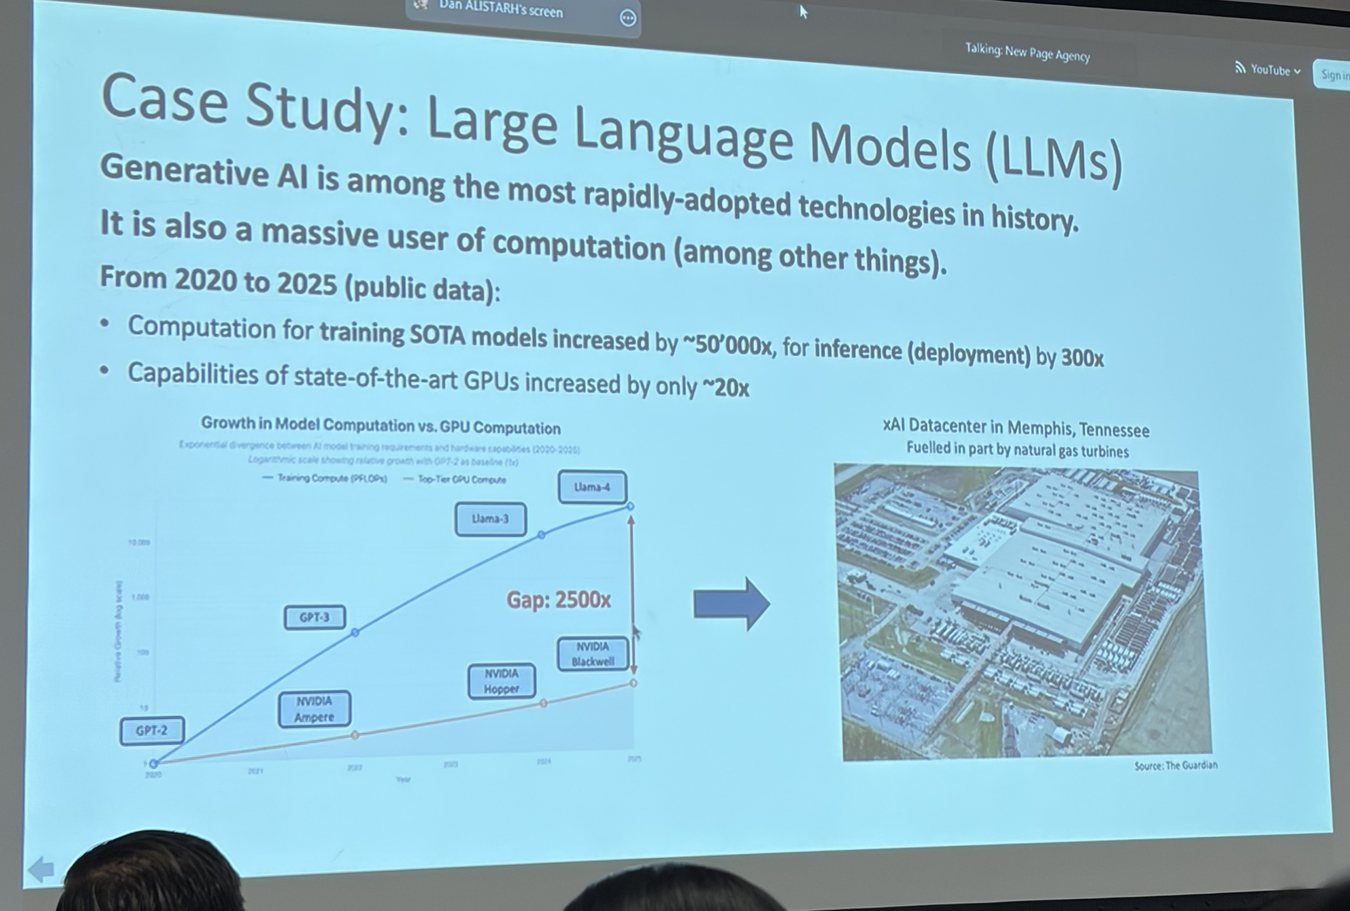
\includegraphics[width=0.86\textwidth]{figures/efficient-learning-1.jpg}
\caption{The argument for the whole lecture, from the Computationally-Efficient Learning slides,
photographed during the talk. Training compute per state-of-the-art model and top-tier GPU
capability are plotted on a log scale with GPT-2 as baseline. The two curves diverge from GPT-2
through GPT-3 to Llama-3 and Llama-4 while the hardware line stays nearly flat across Ampere,
Hopper and Blackwell, leaving the annotated 2500-fold gap. The photograph on the right is the xAI
data centre in Memphis, partly gas-fuelled.}
\label{fig:efficient-learning-1}
\end{figure}

\paragraph{The mathematics is about the loss, not the weights.} This is the load-bearing
derivation and it is short. Quantization is just a particular weight perturbation,
$\mathrm{Compress}(\wt) = \wt + \dw$. Taylor expanding the loss,
\[
  \Loss(\wt + \dw) \approx \Loss(\wt) + \grad_{\wt}\Loss \cdot \dw
    + \tfrac{1}{2}\,\dw\T \Hess\, \dw,
\]
\noindent and since the weights are trained, $\grad_{\wt}\Loss \approx \vect{0}$, so the quantity
actually being minimised is the quadratic form $\tfrac12 \dw\T \Hess \dw$ subject to $\dw$ having
the admissible form $\delta w_i = w_i - \quant(w_i)$ for quantizer $\quant$. For a single weight
the optimum is
\[
  \text{LossImpact}(w_i) = \frac{\bigl(w_i - \quant(w_i)\bigr)^2}{2\,[\Hess\inv]_{ii}},
  \qquad
  \dw^{*} = -\,\frac{w_i - \quant(w_i)}{[\Hess\inv]_{ii}}\; \Hess\inv_{:,i}.
\]
\noindent Two things follow. The cost of rounding a weight is not its rounding error but that
error divided by the corresponding inverse-Hessian entry, so weights differ enormously in how much
they may be moved. And the correction $\dw^{*}$ spreads compensation across the other weights,
which is why good quantizers adjust what they have not yet touched. The lecture attributes this
lineage explicitly to Optimal Brain Damage and Optimal Brain Surgeon, from 1990 and
1993~\citep{lecun1990, hassibi1993}, and to its own scaling in the Optimal Brain Compressor.

\paragraph{Why it becomes practical at LLM scale.} GPTQ and SparseGPT minimise a layer-wise loss
$\norm{\mat{Y}_\ell - \mat{X}_\ell \est{\mat{W}}_\ell}^2$ whose Hessian is
$\mat{X}_\ell \mat{X}_\ell\T$, and the observation that unlocks everything is that this Hessian is
constant with respect to the weights, so it can be precomputed once at the start of
compression~\citep{frantar2023gptq, frantar2023sparsegpt}. The algorithm then sweeps columns of
$\mat{W}_\ell$: quantize column $j$ in saliency order within a block, compute the error, and
update the columns to the right of $j$ using $\dw^{*}$. The supporting machinery is a family of
linear time and space estimators of second-order information at block, layer and global
granularity, with the observation that different models need different granularities.

\paragraph{What the large study actually found.} A million-plus individual task and model
evaluations~\citep{kurtic2025} yield three findings the lecture reduces to one slide. Eight-bit
quantization is essentially lossless. All compression approaches land within roughly 1\% of
baseline on easy benchmarks but degrade more on harder ones, reasoning in particular. And larger
models, 70B and above, are easier to compress and compress more stably across tasks. The study
deliberately restricted itself to schemes with hardware support, W4A16 with INT4 and W8A8 dynamic
per-token with INT8 and FP8, which is what makes the numbers actionable rather than academic.

\paragraph{From measurement to prediction.} The last technical move is to stop measuring the damage
and predict it. The linearity theorem claims that under stated assumptions the effect of
quantization on perplexity is approximately linear in the relative layer-wise squared error,
\[
  \Ex\bigl[\PPL(\est{\mat{W}})\bigr] \approx \PPL(\mat{W}^{*})
    + \sum_{\ell=1}^{L} \alpha_\ell\, t_\ell^{2},
\]
\noindent with $\alpha_\ell$ absolute per-layer constants and $t_\ell$ the $L_2$ error at layer
$\ell$~\citep{malinovskii2025}. The disclaimer is stated on the slide rather than buried: the
theory holds only for methods that do not update weights, so it covers AWQ but not GPTQ. That is a
real limitation, since GPTQ's whole mechanism is the compensating update.

\section*{Notation}

$\wt$ are trained weights, $\dw$ the quantization perturbation, $\quant$ the quantizer, $\Hess$
the Hessian and $\PPL$ perplexity. Note that $\Hess$ here is a Hessian, whereas $\Hcent$ in
Chapter~\ref{ch:02-representational-geometry} is a centring matrix, and the two are kept visually
distinct for exactly that reason.

\section*{Why it matters}

This chapter pairs with the summer school's quantization tutorial, which implements
round-to-nearest and GPTQ against the same mathematics and exhibits the 4-bit failure the findings
predict. It also converges
with Pascanu (Chapter~\ref{ch:07-to-be-figured-out}) on the same diagnosis from a different
direction: Pascanu profiles memory bandwidth and concludes the recurrent block should be cheap,
Alistarh reduces bit-width so the weights fit in faster memory, and both are treating arithmetic
as abundant and data movement as scarce. The lottery ticket citation is shared with
Chapter~\ref{ch:01-intro-deep-learning} under a different interpretation, which is noted there.

\begin{aside}
The framing device deserves attention independently of the content. Alistarh takes the bitter
lesson, which is normally deployed as an argument against clever methods, and derives from it a
mandate for clever methods, on the grounds that if compute is what matters then compute
efficiency is what matters. The move is available whenever a scaling argument is used to dismiss
an idea: ask what the argument implies about the price of the resource it says is decisive.
\end{aside}

\chapter{A Modern Tutorial on Geometric Deep Learning}
\label{ch:11-geometric-deep-learning}

\lecturemeta{Petar Veli\v{c}kovi\'{c}}{Google DeepMind and University of Cambridge}

The organising analogy is historical. In the nineteenth century geometry had fragmented into a
zoo of competing geometries, and Klein's Erlangen Program unified them by asking, for each one,
which group of transformations it leaves invariant. Veli\v{c}kovi\'{c} argues deep learning in the
2020s is in the same position, a zoo of architectures with no principle organising them, and
proposes the same remedy: specify the domain the data lives on and the group of symmetries acting
on it, then derive the admissible layers. The payoff claimed is not aesthetic. For several
architectures the derivation is tight enough to show that they \emph{must} have the form they do,
and the same recipe extends to domains where nobody has intuition, such as spheres and meshes.

\section*{Key ideas}

\paragraph{Invariance, equivariance, and why the second is the useful one.} A function is invariant
if the symmetry leaves its output unchanged, and equivariant if the output transforms
correspondingly. The definition given is that for $f : \dom \to \lab$, a group $\Grp$, and
representations $\rho_1$ and $\rho_2$ acting on the domain and codomain respectively, $f$ is
$\Grp$-equivariant when
\[
  f \circ \rho_1(g) = \rho_2(g) \circ f
  \qquad \text{for all } g \in \Grp,
\]
\noindent so applying the symmetry before $f$ is the same as applying it after. Invariance is the
special case $\rho_2 = \mathrm{id}$. The lecture's point is that
invariance is too strong to build with, because an invariant layer must collapse the whole input to
a single output and thereby throws structure away; so one stacks equivariant layers and takes an
invariant readout only at the end. Whether something is a symmetry is a property of the task, not
of the data: rotation is a symmetry for cats versus dogs and emphatically not for digit
recognition. Groups organise these symmetries, group actions turn them into operations on the
domain, and representations turn the actions into matrices, with $SO(2)$ rotations and $S_3$
permutations as the running examples.

\paragraph{The recipe.} Data lives on a domain $\Om$, an $N \times N$ grid, a set, a graph, and
the data itself is a signal $\Sig : \Om \to \mathcal{C}$. The key structural observation is that
an action on the domain induces an action on signals. Given that, the building blocks are linear
equivariant maps composed with local nonlinearities, and the derivation of each architecture is
just working out which linear maps are equivariant to the group in question. The lecture then works
this through for what it calls the four Gs: graphs, grids, groups and geometric graphs, with
manifolds and gauges as the finale, following the structure of the companion
book~\citep{bronstein2021gdl}.

\paragraph{Graphs give message passing, with no freedom left.} Permutation equivariance plus a
locality requirement forces the layer to be a function of a node and its neighbourhood, and the
result is the message-passing form
\[
  \vect{h}_u = \upd\Bigl(\xin_u, \;\agg_{v \in \nbr{u}} \msg(\xin_u, \xin_v)\Bigr),
\]
\noindent where $\msg$ is the message function, $\agg$ the aggregation and $\upd$ the update
(Figure~\ref{fig:geometric-deep-learning-1}). The only requirement on $\agg$ is permutation
invariance, so sum, max or mean all qualify, and message and update are the only parametric parts.
The lecture is explicit that this is derived rather than designed: locality is presented as
possibly the only way to satisfy equivariance without collapsing.

\begin{figure}[htbp]
\centering
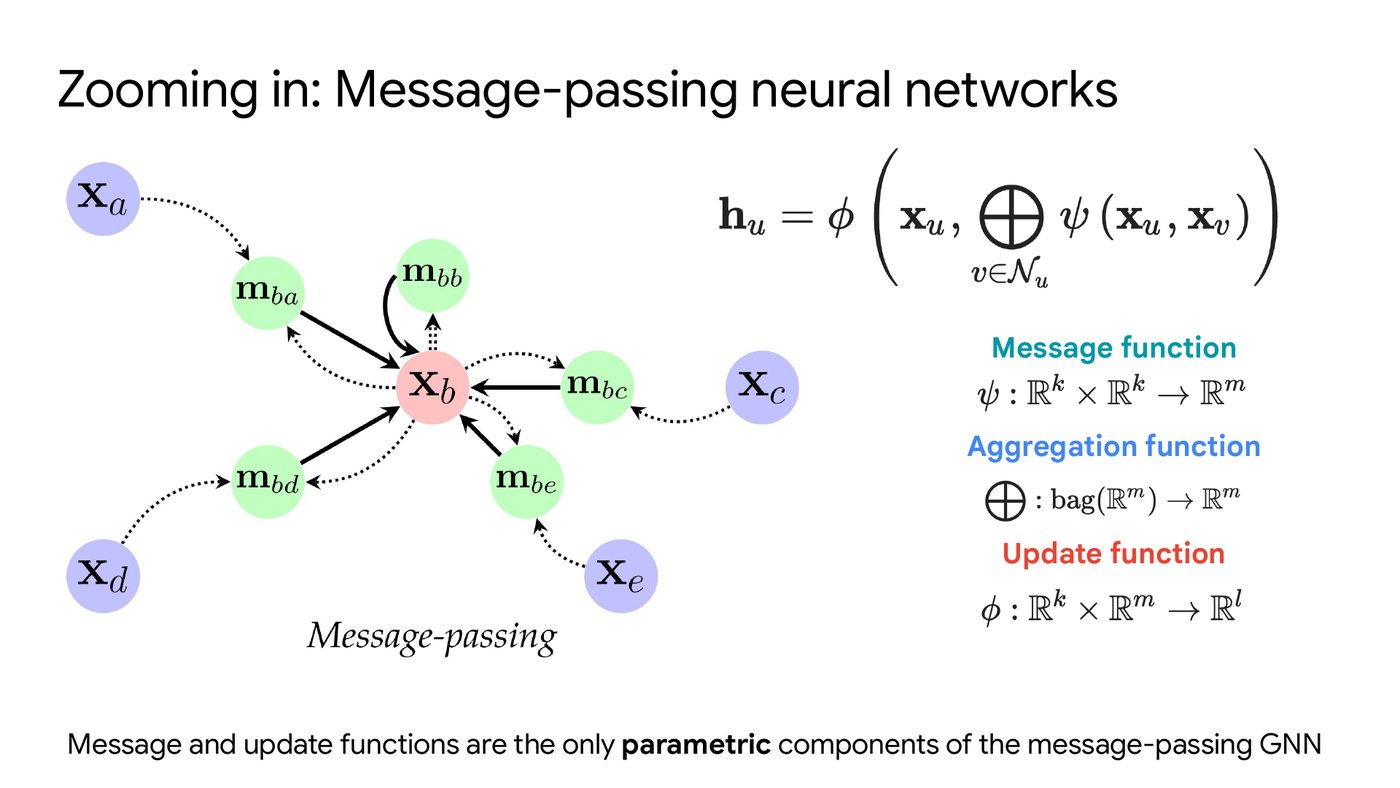
\includegraphics[width=0.86\textwidth]{figures/geometric-deep-learning-1.jpg}
\caption{The message-passing layer as derived in the Geometric Deep Learning tutorial. Node $b$
receives a message $\vect{m}_{bv}$ from each neighbour, the messages are combined by a
permutation-invariant aggregator, and the update produces $\vect{h}_u$. Only $\msg$ and $\upd$ carry
parameters; the aggregator's only job is to make the layer indifferent to neighbour ordering.}
\label{fig:geometric-deep-learning-1}
\end{figure}

\paragraph{Transformers are graph neural networks.} The most provocative section argues that
treating LLMs as sequence models is a category error. Nodes are tokens,
$V = \{1, \dots, N\}$, features are token embeddings, and the causal mask is precisely a
neighbourhood definition, $v \in \nbr{u} \iff v \le u$. Dot-product self-attention is then a
message function in two parts, with the softmax denominator handled by an aggregator that
accumulates both numerator and normaliser and an update that divides, so the whole block is an
MPNN on a complete or causally-masked graph~\citep{joshi2025}, with graph attention
networks~\citep{velickovic2018gat} credited on the slide as the attentional precursor. The practical
value is diagnostic: once a transformer is a GNN, its known pathologies become graph pathologies,
and the lecture names overmixing and oversquashing as exactly the phenomena the GNN literature has
studied. Both connect back to the DAG structure of causal attention in
Chapter~\ref{ch:09-spectral-analysis-dags}.

\begin{figure}[htbp]
\centering
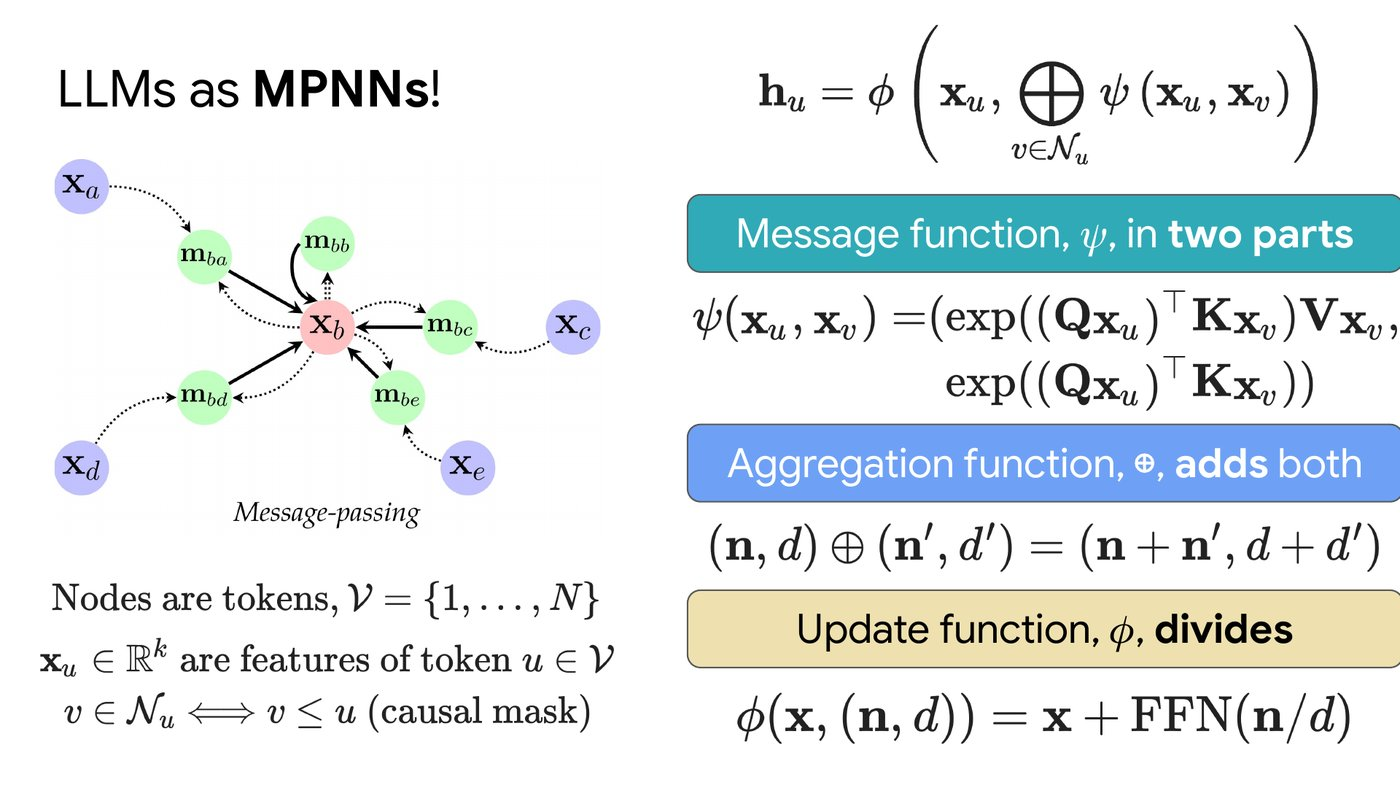
\includegraphics[width=0.86\textwidth]{figures/geometric-deep-learning-2.jpg}
\caption{A transformer block written as message passing, from the Geometric Deep Learning
tutorial. Nodes are tokens, $\nbr{u}$ is fixed by the causal mask $v \le u$, and the block decomposes
exactly into the three MPNN components. The message function carries two parts, the attention
numerator $\exp((\mat{Q}\xin_u)\T \mat{K}\xin_v)\mat{V}\xin_v$ and its denominator
$\exp((\mat{Q}\xin_u)\T \mat{K}\xin_v)$; the aggregator sums both componentwise,
$(\vect{n}, d) \oplus (\vect{n}', d') = (\vect{n} + \vect{n}', d + d')$; and the update performs the
softmax division and the residual feed-forward step,
$\upd(\xin, (\vect{n}, d)) = \xin + \mathrm{FFN}(\vect{n}/d)$.}
\label{fig:geometric-deep-learning-2}
\end{figure}

\paragraph{Grids give CNNs, and the derivation is the point.} A grid is a graph with more
regularity, so one may restrict attention to the special permutations that are translations.
Collecting the parameters of a translation-equivariant linear map into a matrix forces that matrix
to be circulant, and every circulant matrix is a convolution. The conclusion is stronger than
motivation: all linear translation-equivariant maps on a grid are convolutions, which is why CNNs
must have the form they do. The same style of argument recovers gating in recurrent networks from
invariance to time warping, which is a satisfying derivation of GRU and LSTM structure from a
symmetry rather than from engineering.

\paragraph{Groups, and building for domains that resist intuition.} Generalising convolution from
translations to an arbitrary group $\Grp$ gives group convolution~\citep{cohen2016group}, and the
subtlety flagged is that after the first layer the signals live on $\Grp$ rather than on the
original domain, which is what makes depth work. Spheres are the worked example: $\Om = \Sph^2$
with 3D rotation symmetry, layer one maps $\Sph^2 \to SO(3)$ and subsequent layers act on
$SO(3)$~\citep{cohen2018spherical}. The applied highlight is TacticAI
(Figure~\ref{fig:geometric-deep-learning-3}), where the relevant symmetry is the dihedral group
$D_2$, an approximate symmetry of a football pitch under reflection along each
axis~\citep{wang2024tacticai}. This is the result the personal notes record as predicting corner
outcomes several seconds ahead, and the reason it belongs in this lecture is that the pitch
symmetry is approximate, so the equivariance is a modelling choice rather than a fact.

\begin{figure}[htbp]
\centering
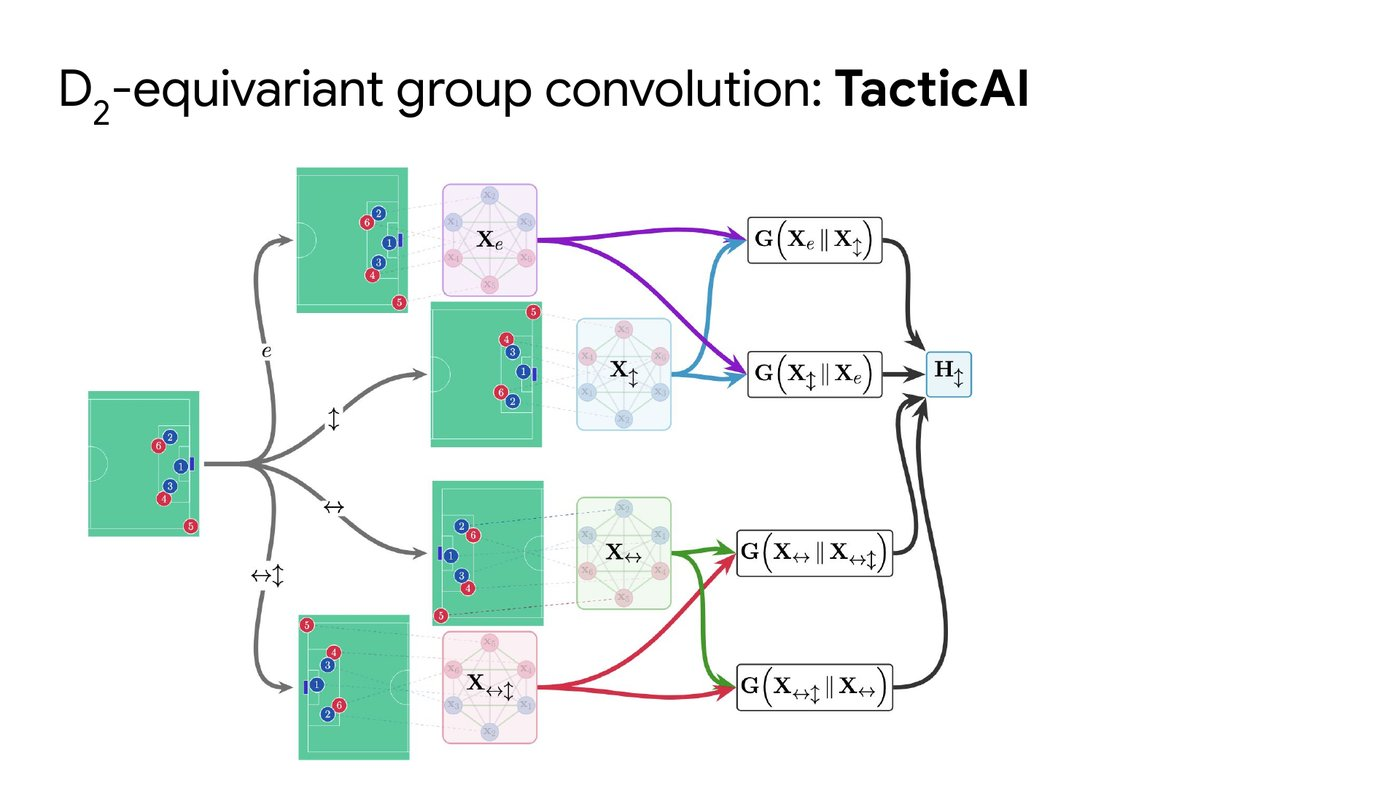
\includegraphics[width=0.88\textwidth]{figures/geometric-deep-learning-3.jpg}
\caption{Group convolution in the wild, from the Geometric Deep Learning tutorial. A corner-kick
configuration is transformed by each element of the dihedral group $D_2$, reflection along the
pitch's long axis, its short axis, and both, giving four views. Each is encoded, the encodings are
combined pairwise, and the result is pooled into a $D_2$-equivariant representation, so the model
cannot give a different answer merely because the play happened on the other side of the pitch.}
\label{fig:geometric-deep-learning-3}
\end{figure}

\paragraph{Geometric graphs, manifolds and gauges.} If the domain does not float in a vacuum but is
embedded in space, the relevant group is $E(3)$, roto-translation and reflection, combined with
permutation equivariance. The cheap route to guaranteed invariance is to message pass only on
invariant quantities such as pairwise distances; vector-valued features need genuinely equivariant
updates instead. Manifolds push this furthest. A 2D manifold is locally like $\R^2$, so one works
in the tangent space $T_u\Om$, moves along the surface with the exponential map $\exp_u X$, and
compares tangent vectors at different points by parallel transport $\Gamma_{u \to v}X$. Defining
convolution in the tangent space then runs into the central difficulty: the choice of gauge, the
local frame, is entirely arbitrary, and even on a sphere no consistent global choice exists.
Requiring gauge equivariance directly means conditioning across pairs of arbitrarily related
gauges, which the lecture calls very hard; parallel transporting features first simplifies it. The
resolution is deflationary and rather satisfying: what results is a GNN with extra precomputations
and angle-conditioned parameters, or as the slide puts it, just a graph with extra
structure. AlphaFold 2 carries the same ideas, maintaining a local frame per residue~\citep{jumper2021}
(Figure~\ref{fig:geometric-deep-learning-4}).

\begin{figure}[htbp]
\centering
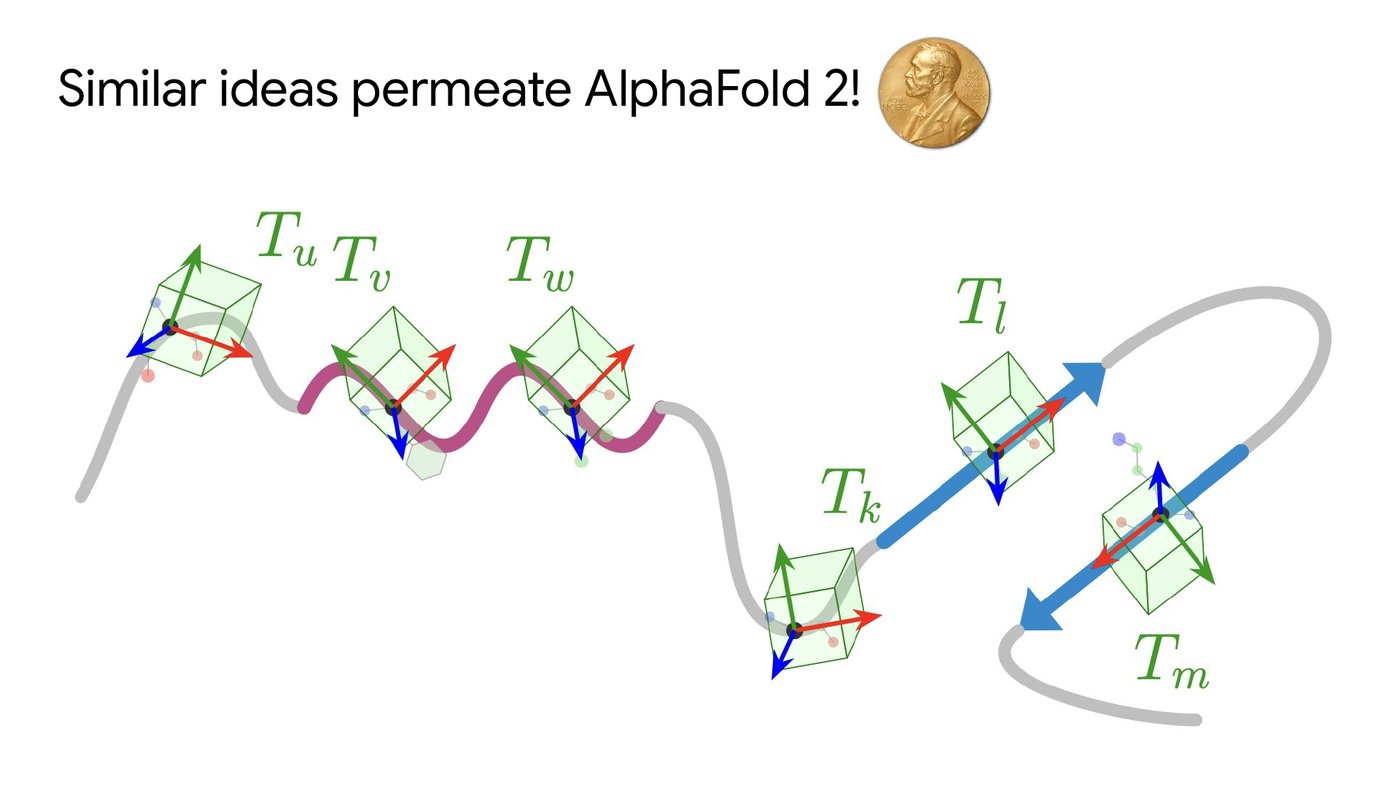
\includegraphics[width=0.82\textwidth]{figures/geometric-deep-learning-4.jpg}
\caption{Where the gauge machinery reappears, from the closing of the Geometric Deep Learning
tutorial. A protein backbone with a local coordinate frame $T_u, T_v, T_w, \dots$ attached to each
residue. Reasoning about relative geometry means transporting information between these frames,
which is the same problem as choosing gauges on a manifold. This is the slide the personal notes
record but whose image attachment is missing from disk; it is recovered here from the deck.}
\label{fig:geometric-deep-learning-4}
\end{figure}

\section*{Notation}

$\Om$ is the domain, $\Sig$ a signal on it, $\Grp$ a group with elements $g$, $\rho$ a
representation, $\nbr{u}$ the neighbourhood of node $u$, and $\msg$, $\agg$, $\upd$ the message,
aggregation and update functions. The slides write $\upd$ as $\phi$ and $\msg$ as $\psi$, and that
usage is kept here. Isola uses $\phi$ for a representation in
Chapter~\ref{ch:02-representational-geometry}, which is an unavoidable collision between two
speakers' conventions.

\section*{Why it matters}

This is the most explicitly unifying lecture of the week and it retroactively organises several
others. Cho's Set Transformer++ (Chapter~\ref{ch:05-statistics-estimation}) is a permutation
equivariant architecture derived exactly the way this lecture prescribes, without either speaker
citing the other. The Feynman-graph failure in
Chapter~\ref{ch:08-ml-for-mathematics}, where $\phi^4$ graphs are 4-regular and so message passing
is blind by 1-WL, is a case where this toolkit is the named fix. And the transformers-as-GNNs claim
is the bridge to Chapter~\ref{ch:09-spectral-analysis-dags}: if a causally-masked transformer is a
GNN on a DAG, then its adjacency spectrum collapses, and zero-padding is a candidate for
recovering it.

\begin{aside}
Two follow-ups from the personal notes belong here. The mathematical prerequisites are published
separately as a long companion on the group- and representation-theoretic background, recorded in
those notes as \url{https://arxiv.org/abs/2508.02723}, and the course home is
\url{https://geometricdeeplearning.com}, with the MIT Press book dated 2026 on the closing slide.
The direction of the dependency is worth noting: nothing in the four Gs requires that background in
order to be \emph{used}, but the derivations, which are the actual content of the lecture, do.
\end{aside}


\part{Synthesis}
\chapter{Cross-cutting Themes}
\label{ch:themes}

Six ideas recurred across the week, and in three cases two speakers reached the same territory from
opposite directions or disagreed outright. A disagreement between people who both know the field
marks an open question rather than a gap in the notes, so those three are the ones to dwell on.

\section*{1. The i.i.d.\ assumption, and a real disagreement about how bad it is}

Chandar closes the opening lecture (Chapter~\ref{ch:01-intro-deep-learning}) by naming the frontier
without explaining it: current practice optimises the i.i.d.\ case, while true learning is
sequential, online and continual. Three later lectures pick that up, and they do not agree.

Lyle (Chapter~\ref{ch:06-continual-learning}) treats it as an engineering fault with an identifiable
mechanism. Plasticity is lost because Adam's second-moment estimate is stale after a task change, so
the effective step size explodes, and because a large step pushes preactivations outside the
receptive field of the nonlinearity. Both are fixable by normalising, controlling parameter
norm, and avoiding regression on ill-conditioned targets, with resetting and distilling as a
fallback. Her verdict on forgetting is even more deflationary: if the data can be kept, the problem
is easy.

Pascanu (Chapter~\ref{ch:07-to-be-figured-out}) makes a structural claim instead. Gradient-based
credit assignment works by tug-of-war dynamics between competing examples, and that mechanism
\emph{requires} shuffled data. On this reading catastrophic forgetting is not a side effect but is
what failed credit assignment looks like, and Lyle's fixes are palliative because they stabilise
training without giving the learner explicit knowledge composition. He offers as hypotheses that
there is no compositional knowledge in these models and that scale is a crutch making learning
possible at all.

Deac's tutorial material (Chapter~\ref{ch:04-intro-reinforcement-learning}) is the third data point
and it supports Pascanu quietly: experience replay exists precisely because consecutive transitions
are correlated and SGD assumes independence. Replay is continual learning solved by refusing to be
in the continual setting, which is exactly Lyle's advice, and it is also an admission that nobody
knows how to learn from a correlated stream directly.

The disagreement is testable, which is what makes it interesting;
Chapter~\ref{ch:research-directions} sketches an experiment that would separate the two positions.

\section*{2. Symmetry imposed versus symmetry measured}

Veli\v{c}kovi\'{c} (Chapter~\ref{ch:11-geometric-deep-learning}) and Isola
(Chapter~\ref{ch:02-representational-geometry}) are doing the same thing from opposite ends.
Veli\v{c}kovi\'{c} specifies the symmetry group first and derives which layers are admissible,
strongly enough that CNNs are shown to be the only linear translation-equivariant maps on a grid.
Isola takes trained networks and measures, after the fact, which transformations their
representations are invariant to, then argues the right equivalence is isometry because distance is
what downstream tasks consume. One prescribes the invariance, the other discovers it.

The most striking evidence that this is one idea rather than two is that Cho
(Chapter~\ref{ch:05-statistics-estimation}) derives a permutation-equivariant architecture, a
transformer with positional embeddings removed, from exactly Veli\v{c}kovi\'{c}'s reasoning, in a
lecture about statistics, without either speaker referencing the other. The same argument
arriving independently in three lectures is some evidence it is not incidental.

\section*{3. Where knowledge gets injected}

Three lectures address the same question: if a model cannot learn everything from data, where does
the rest come from?

Cho's answer is to stop modelling the generative process. Inference need not invert generation, so an
estimator can be trained directly on problems with known answers, at the price of making
identifiability relative to the prior over problems, the hypothesis space and the optimiser. Pascanu's
answer is the mirror image: there is no prior-free machine learning system, every construction step
is a bias, so the question is never whether to encode knowledge but which encoding pays. And
Tapu\v{s}kovi\'{c} (Chapter~\ref{ch:08-ml-for-mathematics}) locates it in the evaluator, arguing that
in the 67-problem study search was never the bottleneck and that building a cheap, exact,
ungameable score \emph{is} the research.

Isola sits awkwardly across this. His lecture uses fixed metrics such as CKA to establish that
models converge, but his stated opinion is that there is no future for distance functions that are
not learned. Taken together with Cho, that points somewhere uncomfortable: if both the model and
the yardstick are fitted, convergence results become hard to state without circularity.

\section*{4. The spectrum as the design surface}

Three unrelated lectures turn out to be doing spectral engineering. Dieleman
(Chapter~\ref{ch:03-diffusion-models}) explains why diffusion works on images by observing that
natural images have a decaying power spectrum while Gaussian noise is flat, so the noise schedule is
effectively a frequency schedule and sampling recovers bands coarsest-first. Stankovi\'{c}
(Chapter~\ref{ch:09-spectral-analysis-dags}) cannot filter on a DAG at all until a spectrum is
restored, because nilpotency collapses every eigenvalue to zero. And Pascanu's linear recurrent unit
is designed entirely in the spectral domain, with the eigenvalue modulus setting the memory horizon
and the initialisation annulus chosen so that no unit begins with a memory too short to matter.

In all three the eigenvalues are not a diagnostic applied afterwards; they are the thing being
chosen.

\section*{5. Arithmetic is cheap, moving data is not}

Alistarh (Chapter~\ref{ch:10-efficient-learning}) and Pascanu converge on one conclusion from
opposite directions. Alistarh's framing is a 2500-fold gap between compute demand and hardware
capability over five years, and his remedy is to reduce bit-width so that weights occupy less of the
scarce resource. Pascanu profiles a TPU, finds roughly an eightfold gap between HBM and VMEM
transfer rates, and concludes the recurrent block should be cheap because the memory traffic
dominates. Neither is optimising FLOPs. Both treat arithmetic as abundant and data movement as the
constraint. The first question in any efficiency work is what has to move, not how many operations
there are.

\section*{6. Transformers are not what we call them}

Three lectures reframe the same architecture, and the reframings are compatible.
Veli\v{c}kovi\'{c} argues transformers are graph neural networks and not sequence models, with tokens
as nodes and the causal mask as a neighbourhood, which makes overmixing and oversquashing inherited
graph pathologies rather than novel LLM problems. Stankovi\'{c} notes in passing that a causal
attention mask is a strictly upper triangular matrix, hence a DAG, hence spectrally degenerate.
Pascanu argues transformers are a factorisation into simple components that must be scaled, and that
attention might not be all we need, while also reporting honestly that the hybrid alternative
retains 25\% global softmax attention because pure recurrence loses on language.

Read together they say the architecture is better understood as a message-passing operator on a
particular graph than as a sequence model, and that its known limitations follow from that graph.

\begin{aside}
One theme is conspicuous by its absence. Nobody argued for scale as a sufficient answer. Alistarh
opens with the bitter lesson and immediately derives a mandate for efficiency from it; Pascanu says
scale might work but is not the only option; Tapu\v{s}kovi\'{c} reports that the tool beats the
literature only where the literature is thin. That is a summer school's selection effect as much as a fact
about the field, but it is consistent across eleven speakers.
\end{aside}

\chapter{Research Directions}
\label{ch:research-directions}

Each item below is attributed to where it came from. Items marked \textbf{flagged} were named as
open by the speaker. Items marked \textbf{inferred} are editorial, drawn from placing two lectures
next to each other, and should be treated as untested conjecture rather than as anything the
speakers endorsed.

\section*{Problems the speakers explicitly left open}

\paragraph{Measuring what we care about when building a representation. Flagged, Pascanu
(Chapter~\ref{ch:07-to-be-figured-out}).} He argues that non-i.i.d.\ structure cannot be exploited
because we do not know how to measure representation quality during training, and separately because
learning lacks compositionality and locality. The measurement problem is the tractable half: it is a
concrete request for a training-time signal that predicts downstream representation quality.

\paragraph{Evaluating continual learning at all. Flagged, Lyle
(Chapter~\ref{ch:06-continual-learning}).} She states the meta-problem plainly and neither option is
acceptable: a pre-specified task sequence is artificial, a naturally continual application is
uncontrolled. Any result in the field inherits this weakness, so a defensible evaluation protocol
would be a contribution in itself.

\paragraph{In-context learning as a continual learning mechanism. Flagged, Lyle.} Her closing slide
calls this an exciting paradigm that brings its own challenges, without saying which. Given the rest
of her lecture, the obvious question is whether in-context adaptation escapes the plasticity problem
or merely relocates it into the context window.

\paragraph{What else admits a learned estimator. Flagged, Cho
(Chapter~\ref{ch:05-statistics-estimation}).} Asked directly on a slide. He has done population
standard deviation, mutual information, Bayesian predictive distributions and causal effects. The
programme's requirement is a simulator of problems with known answers, which is the real filter on
what comes next.

\paragraph{Whether a world model aligns the way vision and language models do. Flagged, Isola
(Chapter~\ref{ch:02-representational-geometry}).} Posed as an open question on a slide. His
convergence results are for vision and language; whether a model trained on interaction and dynamics
lands on the same kernel is untested and would discriminate between the three hypotheses he offers
about what "same" means.

\paragraph{Generalisation in diffusion models, and flow maps. Flagged, Dieleman
(Chapter~\ref{ch:03-diffusion-models}).} His closing slide lists what he did not cover:
generalisation versus memorisation, integrating diffusion models via flow
maps~\citep{dieleman2026flowmaps}, reward-based steering and finetuning, and multimodal generative
models. The flow-maps thread is also flagged in the personal notes.

\paragraph{Quantized training, and extending the linearity theorem. Flagged, Alistarh
(Chapter~\ref{ch:10-efficient-learning}).} He names quantized training as the frontier and says big
open questions sit at the intersection of representations, optimisation and compute. There is also a
precise gap on the slide: the linearity theorem holds only for methods that do not update weights, so
it covers AWQ but not GPTQ, which is awkward because GPTQ's compensating update is its whole
mechanism.

\paragraph{Building faithful evaluators, and learning a Galois action. Flagged,
Tapu\v{s}kovi\'{c} (Chapter~\ref{ch:08-ml-for-mathematics}).} His stated conclusion is that search is
not the bottleneck and constructing a cheap, exact, ungameable score is the research. He also asks
directly whether the action of the Cosmic Galois Group on Feynman Mellin motives can be learned, and
observes that machine certification stops exactly where the deep objects begin, which is a diagnosis
of where formalisation effort should go.

\paragraph{Gauge equivariance without parallel transport. Flagged, Veli\v{c}kovi\'{c}
(Chapter~\ref{ch:11-geometric-deep-learning}).} Conditioning across arbitrarily related pairs of
gauges is described as very hard, and the working solution sidesteps it by transporting features
first. Whether the harder formulation buys anything is open.

\paragraph{Why real-world reinforcement learning fails. Flagged, Deac
(Chapter~\ref{ch:04-intro-reinforcement-learning}).} Her own live bandit collected zero votes over 53
rounds, and the closing slide enumerates the causes: reward confounded with content,
non-stationarity, sparsity, noise, varying turnout, delayed and batched feedback, and a false
independence assumption across action dimensions. That list is a better research agenda than most
papers' future-work sections.

\section*{Directions inferred here, not reported}

\paragraph{Give causally-masked transformers a spectrum. Inferred, from Stankovi\'{c} and
Veli\v{c}kovi\'{c}.} Stankovi\'{c} notes that a causal attention mask is strictly upper triangular and
therefore nilpotent, and Veli\v{c}kovi\'{c} argues a transformer \emph{is} a GNN on that graph. Putting
the two together, every decoder-only transformer is a graph whose adjacency spectrum has collapsed,
and her zero-padding construction is a candidate for restoring it: add a return path with enough zero
tokens that the induced feedback cannot reach real tokens within the depth of the network. Whether
the restored spectrum says anything useful about attention is entirely untested, and the construction
was designed for graph filters rather than learned attention, so this may not survive contact.

\paragraph{An experiment that would separate Lyle from Pascanu. Inferred.} Lyle claims plasticity
loss is a fixable optimiser and architecture fault; Pascanu claims gradient-based credit assignment
structurally needs i.i.d.\ data. Apply Lyle's full remedy, normalisation, norm control, avoiding
ill-conditioned targets, and then test not whether training remains stable, which she has shown, but
whether knowledge \emph{composes}: does a model trained on tasks $A$ then $B$ solve compositions of
$A$ and $B$ better than one trained on $B$ alone? Lyle's account predicts that stability suffices;
Pascanu's predicts that composition still fails. No such experiment appears in either lecture.

\paragraph{A learned representational similarity metric. Inferred, from Cho and Isola.} Isola says
unlearned distance functions have no future; Cho shows how to learn an estimator whenever problems
with known answers can be simulated. Representational similarity is a candidate: train an estimator
on pairs of representations related by known transformations, with the transformation as the label.
The hazard is the circularity flagged in Chapter~\ref{ch:themes}: convergence results measured with
a fitted metric are hard to interpret, and confronting that directly might be the more valuable
output.

\paragraph{Model the compensating update in the linearity theorem. Inferred, from Alistarh.} The
theorem's disclaimer excludes weight-updating methods. GPTQ's update is not arbitrary though: it is
the closed-form $\dw^{*}$ from the inverse Hessian. That suggests the theorem might extend by
carrying the update through the per-layer error term rather than by treating it as unmodelled noise.
Speculative, and whether the assumptions survive has not been checked.

\begin{aside}
Every item in the second list is a guess made by putting two lectures side by side, and none of them
was checked against the literature. Anyone who finds that one of them has already been done, or is
already known not to work, is better informed than these notes are.
\end{aside}

\chapter{Worth Revisiting}
\label{ch:revisit}

Thirteen things from the week that reward a second pass, in no particular order. Some are readings,
some are exercises, and a few are loose ends that nobody has tied up.

\begin{enumerate}

\item \textbf{The 4-bit failure in the quantization tutorial}, in the section headed 8-bit RTN.
  Round-to-nearest quantization is essentially lossless at 8 bits and visibly destroys the same model
  at 4. Watching that happen before reading Chapter~\ref{ch:10-efficient-learning} is what makes the
  inverse-Hessian derivation feel necessary rather than decorative.

\item \textbf{Activation steering}, exercises 9 to 11 of the mechanistic interpretability tutorial.
  A steering vector is built from the contrast between two sets of prompts, added to the residual
  stream mid-generation, and the effect on the output is unmistakable. The whole method fits in three
  exercises and transfers to any model that can be wrapped in TransformerLens.

\item \textbf{Continual learning, read as a disagreement.} Chapter~\ref{ch:06-continual-learning}
  and then Chapter~\ref{ch:07-to-be-figured-out}. Lyle treats plasticity loss as a fixable fault in
  the optimiser and the architecture; Pascanu treats the same territory as evidence that
  gradient-based credit assignment structurally depends on i.i.d.\ data. Reading them in that order
  makes the gap between the two positions visible in a way neither lecture does alone.

\item \textbf{Dieleman on diffusion as spectral autoregression},
  \url{https://sander.ai/2023/07/20/perspectives.html}. The slide version, Figure~\ref{fig:diffusion-models-3}, compresses
  the argument to four panels. The post carries the derivation, and it is the most reusable idea in
  the diffusion lecture: the noise schedule is a frequency schedule.

\item \textbf{PPO and GRPO, implemented in that order}, Part~2 of the reinforcement learning
  tutorial. PPO is built first with a critic, at full memory cost, and GRPO then removes the critic
  in a few lines by standardising rewards within a sampled group. The ordering is what makes GRPO's
  appeal legible rather than merely stated.

\item \textbf{The Kazhdan--Lusztig experiment}~\citep{davies2021}, with
  Chapter~\ref{ch:08-ml-for-mathematics}. Gradient attribution on a trained GNN flagged particular
  edges, those edges suggested a decomposition, and the decomposition became a conjecture. It is the
  clearest example available of a model's internals being legible enough to turn into a mathematical
  statement.

\item \textbf{The linear recurrent unit derivation, all six steps.} \citet{orvieto2023}, with
  Chapter~\ref{ch:07-to-be-figured-out}. An ablation dressed as an architecture, where the negative
  results are the substance: HiPPO is unnecessary, continuous time is unnecessary, and complex
  numbers may buy nothing beyond compactness. A better first reading on state space models than most
  explainers.

\item \textbf{CKA and the invariance argument around it}~\citep{kornblith2019}, with
  Chapter~\ref{ch:02-representational-geometry}. A small formula with a great deal of thinking behind
  it. The transferable habit is to ask of any similarity measure which transformations it has been
  built to ignore, and whether those are the ones the downstream task ignores too.

\item \textbf{The eight-episode TD versus Monte Carlo exercise.} Slides 37 to 39 of the
  reinforcement learning deck, with Chapter~\ref{ch:04-intro-reinforcement-learning}. Five minutes
  with pen and paper, and it fixes the difference between fitting the observed data and fitting the
  model that data implies. Best attempted before looking at the answer.

\item \textbf{Computational identifiability.} Chapter~\ref{ch:05-statistics-estimation}, final
  section, and~\citet{bynum2026identifiability}. Identifiability defined relative to a prior over
  problems, a hypothesis space and an optimiser, rather than absolutely. The idea from the week most
  likely to change how a problem is framed rather than how it is solved.

\item \textbf{Zero-padding applied to causal attention.}
  Chapter~\ref{ch:09-spectral-analysis-dags}, with the inferred direction in
  Chapter~\ref{ch:research-directions}. A causally-masked transformer is a DAG, so its adjacency
  spectrum collapses. Whether Stankovi\'{c}'s construction says anything useful about attention is
  untested, and cheap to sanity-check on a small mask.

\item \textbf{PECNET with a state space model}, presented at the poster session by Mustafa Abdullah
  Hakkoz for regional agricultural forecasting. Worth pairing with the state space material in
  Chapter~\ref{ch:07-to-be-figured-out}, since the poster puts a hybrid to work on a real forecasting
  problem rather than on a benchmark.

\item \textbf{The geometric deep learning prerequisites},
  \url{https://arxiv.org/abs/2508.02723}, with the course at
  \url{https://geometricdeeplearning.com}. The group- and representation-theoretic background is not
  needed to apply the four Gs, only to derive them. Time well spent for anyone intending to build an
  architecture from a symmetry rather than pick one off the shelf.

\end{enumerate}


\backmatter
\printbibliography[heading=bibintoc,title={References}]

\end{document}
